\documentclass[11pt,a4paper]{article}
\usepackage[utf8]{inputenc}
\renewcommand{\tablename}{Tabla}
\renewcommand{\figurename}{Figura}
\renewcommand{\contentsname}{Índice}
\usepackage{amsmath,amssymb,amsthm}
\usepackage{booktabs}
\usepackage{tabularx}
\usepackage{geometry}
\geometry{a4paper, margin=1in, top=1.2in, bottom=1.2in}
\usepackage{hyperref}
\hypersetup{
    colorlinks=true,
    linkcolor=blue,
    citecolor=blue,
    urlcolor=blue,
    pdftitle={Estadistica II - Guia Basada en Ejemplos - Capitulo 5 - Ajuste de Curvas y Regresion},
    pdfauthor={Gemini Notebook}
}
\usepackage{xcolor}
\usepackage{tcolorbox}
\usepackage{fancyhdr}
\usepackage{graphicx}
\newcommand{\grafico}[2][0.75\textwidth]{%
  \IfFileExists{#2}{\includegraphics[width=#1]{#2}}{%
    \fbox{\parbox[c][3.5cm][c]{#1}{\centering\small
    Archivo gráfico no disponible: \texttt{\detokenize{#2}}}}}}
\usepackage{longtable}
\usepackage{lscape}
\usepackage{enumitem}
\usepackage{tikz}
\usetikzlibrary{arrows.meta,positioning,shapes.geometric,fit}
\usepackage{pgfplots}
\pgfplotsset{compat=1.18}

\tikzset{
  decision/.style={diamond,draw=orange!80!black,fill=orange!8,thick,
    text width=3.1cm,align=center,inner sep=2pt,aspect=2},
  proceso/.style={rectangle,rounded corners=2mm,draw=blue!70!black,fill=blue!5,thick,
    text width=3.5cm,minimum height=1.05cm,align=center},
  resultado/.style={rectangle,rounded corners=2mm,draw=green!55!black,fill=green!5,thick,
    text width=3.5cm,minimum height=1.05cm,align=center},
  alerta/.style={rectangle,rounded corners=2mm,draw=red!65!black,fill=red!5,thick,
    text width=3.5cm,minimum height=1.05cm,align=center},
  flujo/.style={-{Stealth[length=2.3mm]},thick,draw=gray!75},
  etiqueta/.style={font=\scriptsize,fill=white,inner sep=1pt}
}

\pagestyle{fancy}
\fancyhf{}
\fancyhead[L]{\small \bfseries Estadística II: Guía Práctica de Estudio}
\fancyhead[R]{\small \bfseries Capítulo 5: Ajuste de Curvas y Regresión}
\fancyfoot[C]{\thepage}
\fancyfoot[R]{\small\itshape Universidad de Mendoza}
\renewcommand{\headrulewidth}{0.6pt}
\renewcommand{\footrulewidth}{0.4pt}

\newtcolorbox{importante}[1][]{
    colback=red!5!white,
    colframe=red!75!black,
    fonttitle=\bfseries,
    title=Atención - Error Frecuente,
    #1
}

\newtcolorbox{guion}[1][]{
    colback=blue!5!white,
    colframe=blue!75!black,
    fonttitle=\bfseries,
    title=Guion de Exposición Oral,
    #1
}

\newtcolorbox{ejemplo}[1][]{
    colback=yellow!5!white,
    colframe=yellow!60!black,
    fonttitle=\bfseries,
    title=Ejemplo Integrador,
    #1
}

\newtcolorbox{consejo}[1][]{
    colback=green!5!white,
    colframe=green!75!black,
    fonttitle=\bfseries,
    title=Pregunta de Examen / Razonamiento,
    #1
}

\newtcolorbox{ruta}[1][]{
    colback=blue!3!white,
    colframe=blue!65!black,
    fonttitle=\bfseries,
    title=Ruta rápida de estudio,
    boxsep=1mm,left=1.5mm,right=1.5mm,top=1mm,bottom=1mm,
    #1
}

\setlist[itemize]{topsep=2pt,itemsep=1.5pt,parsep=0pt}
\setlist[enumerate]{topsep=2pt,itemsep=2pt,parsep=0pt}
\renewcommand{\arraystretch}{1.15}

% lscape gira el contenido, pero no informa la orientación al visor PDF.
% Este entorno agrega la rotación de página para que se abra apaisada.
\newenvironment{paisaje}{%
  \begin{landscape}\pdfpageattr{/Rotate 90}%
}{%
  \end{landscape}\pdfpageattr{/Rotate 0}%
}

\begin{document}
\hypersetup{pageanchor=false}

% -------------------------------------------------------------
% PORTADA
% -------------------------------------------------------------
\begin{titlepage}
    \centering
    \vspace*{1.5cm}
    {\scshape\LARGE Universidad de Mendoza \par}
    \vspace*{0.5cm}
    {\scshape\Large Cátedra de Estadística Aplicada II \par}
    \vspace*{1.5cm}
    {\Huge\bfseries CAPÍTULO 5: AJUSTE DE CURVAS \\ Y REGRESIÓN \par}
    \vspace*{0.8cm}
    {\Large\itshape Guía de Estudio Práctica y Teórica Basada en Ejemplos Reales para el Examen Final Oral \par}
    \vspace*{1.5cm}
    \vfill
    \begin{tcolorbox}[colback=blue!5!white,colframe=blue!40!black,title=Enfoque Pedagógico de esta Guía]
        Esta guía de estudio aborda los temas del Capítulo 5 partiendo directamente de situaciones reales y ejercicios prácticos de la cátedra. A través de la visualización gráfica y la deducción paso a paso, el estudiante comprenderá primero el problema práctico, luego el razonamiento intuitivo y finalmente la formalización matemática para asegurar una exposición oral fluida ante el tribunal examinador.
    \end{tcolorbox}
    \vfill
    {\large Agosto de 2026 \par}
\end{titlepage}
\hypersetup{pageanchor=true}
\newpage

% -------------------------------------------------------------
% ÍNDICE Y TEMARIO
% -------------------------------------------------------------
\tableofcontents
\newpage

% -------------------------------------------------------------
% MAPA GENERAL DE DECISIÓN
% -------------------------------------------------------------
\begin{paisaje}
\thispagestyle{plain}
\section*{Mapa general de decisión de la Unidad 5}
\addcontentsline{toc}{section}{Mapa general de decisión de la Unidad 5}
\begin{center}
\resizebox{0.95\linewidth}{0.72\textheight}{%
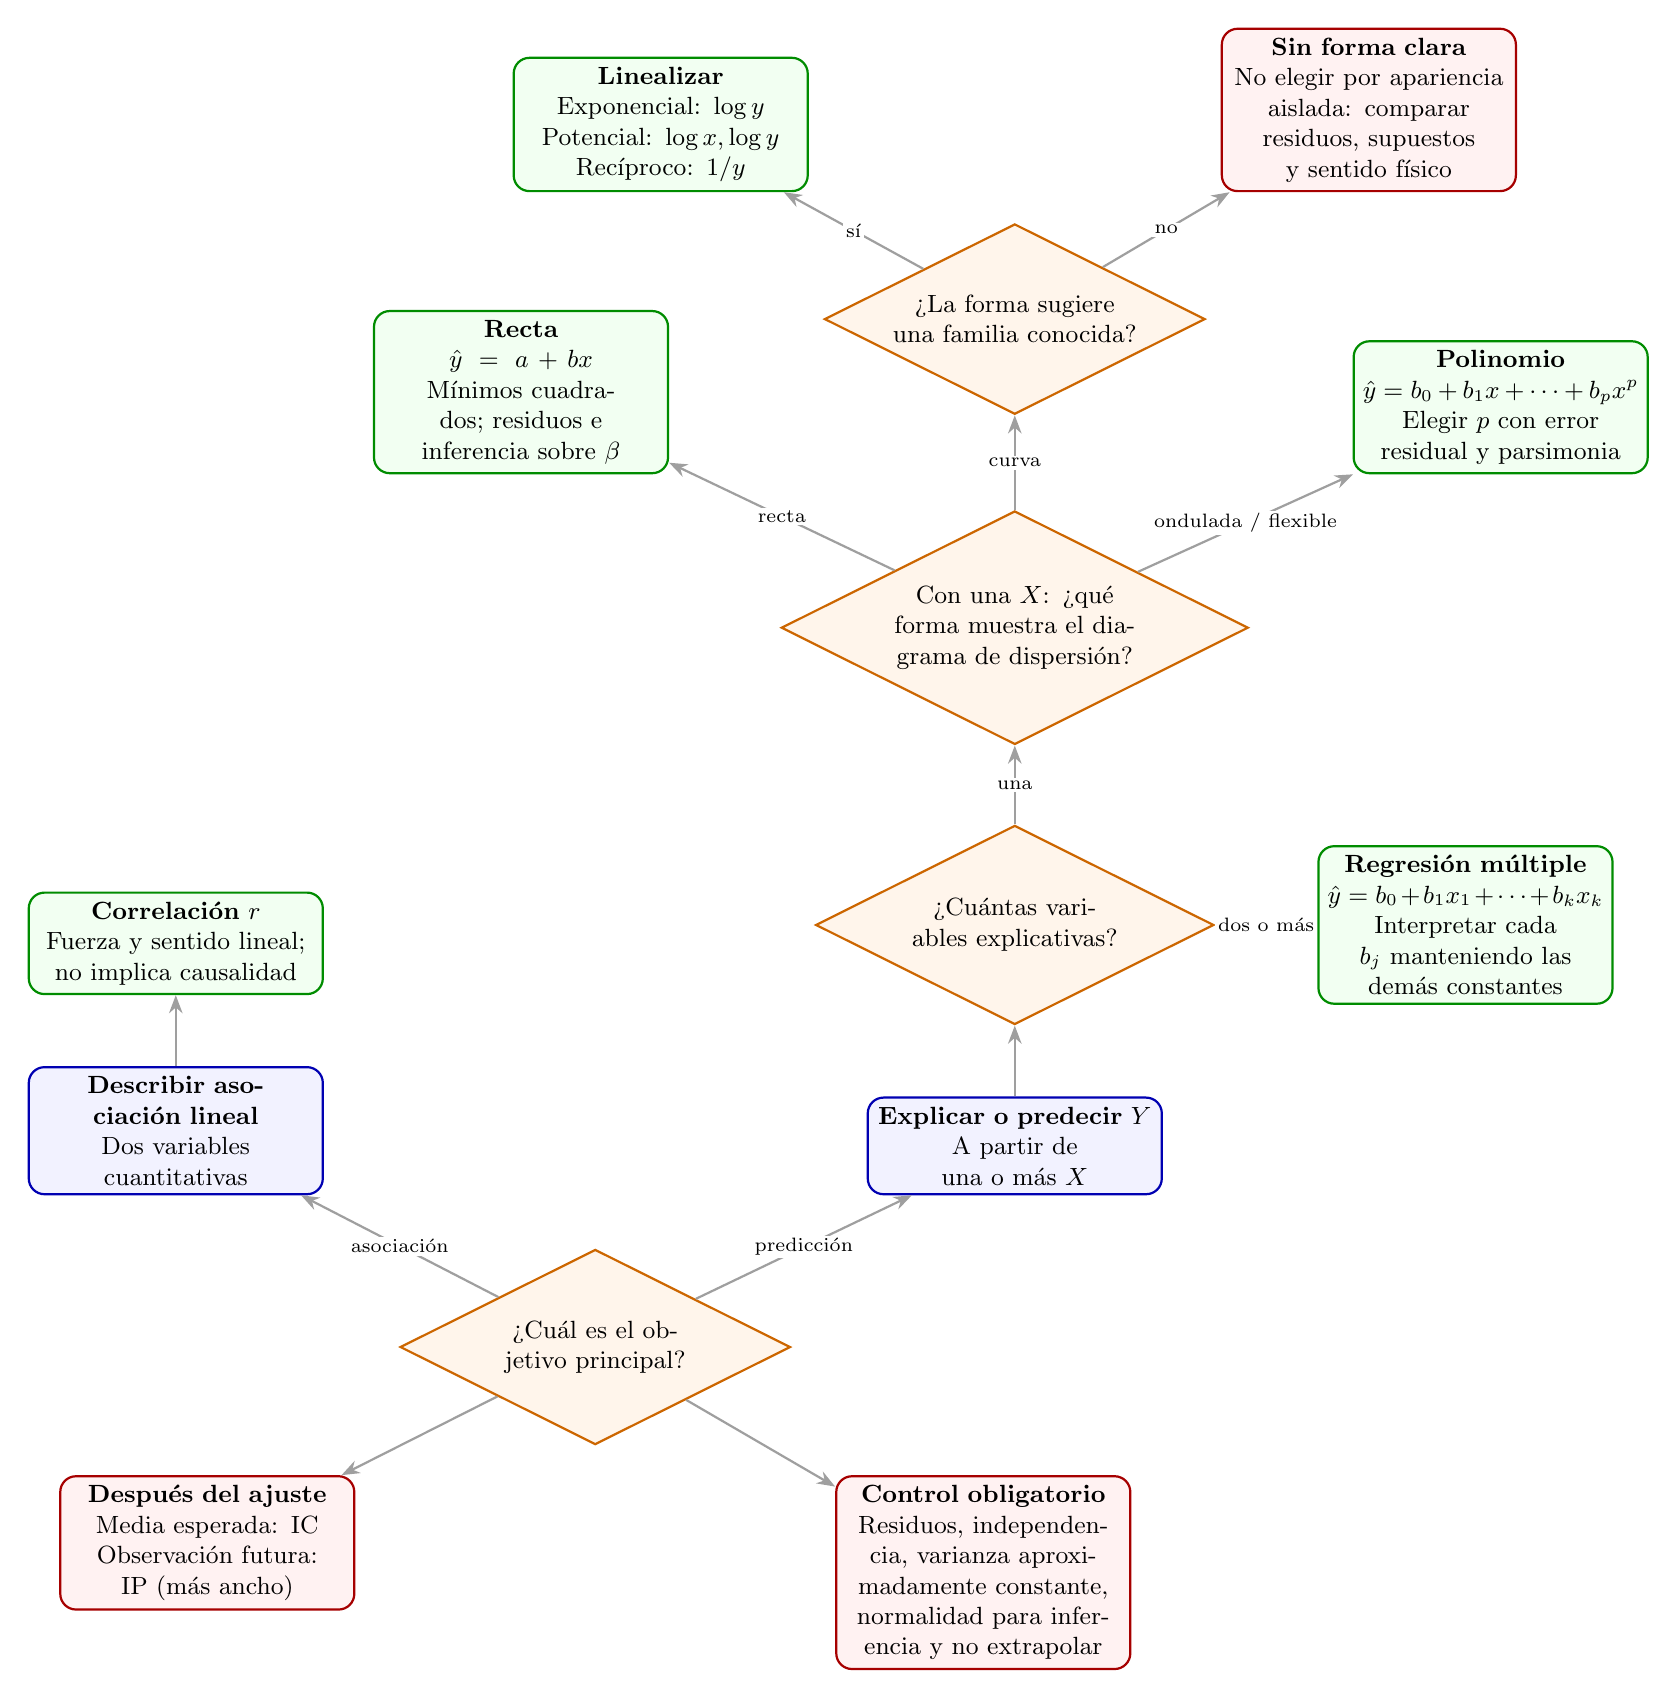
\begin{tikzpicture}[font=\small,node distance=8mm and 11mm]
\node[decision,text width=3.2cm] (objetivo) {¿Cuál es el objetivo principal?};
\node[proceso,above left=13mm and 22mm of objetivo] (asoc) {\textbf{Describir asociación lineal}\\Dos variables cuantitativas};
\node[proceso,above right=13mm and 22mm of objetivo] (pred) {\textbf{Explicar o predecir $Y$}\\A partir de una o más $X$};
\node[resultado,above=9mm of asoc] (corr) {\textbf{Correlación $r$}\\Fuerza y sentido lineal; no implica causalidad};
\node[decision,above=9mm of pred,text width=3.3cm] (cuantas) {¿Cuántas variables explicativas?};
\node[resultado,right=13mm of cuantas] (multiple) {\textbf{Regresión múltiple}\\$\hat y=b_0+b_1x_1+\cdots+b_kx_k$\\Interpretar cada $b_j$ manteniendo las demás constantes};
\node[decision,above=10mm of cuantas,text width=3.4cm] (forma) {Con una $X$: ¿qué forma muestra el diagrama de dispersión?};
\node[resultado,above left=12mm and 29mm of forma] (lineal) {\textbf{Recta}\\$\hat y=a+bx$\\Mínimos cuadrados; residuos e inferencia sobre $\beta$};
\node[decision,above=12mm of forma,text width=3.2cm] (curva) {¿La forma sugiere una familia conocida?};
\node[resultado,above right=12mm and 28mm of forma] (poli) {\textbf{Polinomio}\\$\hat y=b_0+b_1x+\cdots+b_px^p$\\Elegir $p$ con error residual y parsimonia};
\node[resultado,above left=10mm and 14mm of curva] (transf) {\textbf{Linealizar}\\Exponencial: $\log y$\\Potencial: $\log x,\log y$\\Recíproco: $1/y$};
\node[alerta,above right=10mm and 14mm of curva] (diag) {\textbf{Sin forma clara}\\No elegir por apariencia aislada: comparar residuos, supuestos y sentido físico};
\node[alerta,below left=10mm and 18mm of objetivo] (intervalos) {\textbf{Después del ajuste}\\Media esperada: IC\\Observación futura: IP (más ancho)};
\node[alerta,below right=10mm and 18mm of objetivo] (control) {\textbf{Control obligatorio}\\Residuos, independencia, varianza aproximadamente constante, normalidad para inferencia y no extrapolar};
\draw[flujo](objetivo)--node[etiqueta]{asociación}(asoc);
\draw[flujo](asoc)--(corr);
\draw[flujo](objetivo)--node[etiqueta]{predicción}(pred);
\draw[flujo](pred)--(cuantas);
\draw[flujo](cuantas)--node[etiqueta]{dos o más}(multiple);
\draw[flujo](cuantas)--node[etiqueta]{una}(forma);
\draw[flujo](forma)--node[etiqueta]{recta}(lineal);
\draw[flujo](forma)--node[etiqueta]{curva}(curva);
\draw[flujo](forma)--node[etiqueta]{ondulada / flexible}(poli);
\draw[flujo](curva)--node[etiqueta]{sí}(transf);
\draw[flujo](curva)--node[etiqueta]{no}(diag);
\draw[flujo](objetivo)--(intervalos);
\draw[flujo](objetivo)--(control);
\end{tikzpicture}}
\end{center}
\vfill
\begin{tcolorbox}[colback=gray!4,colframe=gray!55,title=Lectura rápida para el examen]
\small Primero defina el objetivo y el diseño; después observe la forma, ajuste el modelo y controle los residuos. Un $R^2$ o un $|r|$ alto no reemplaza el diagnóstico, no demuestra causalidad y no autoriza extrapolar fuera del rango observado.
\end{tcolorbox}
\end{paisaje}
\newpage

\section{Temario Oficial del Capítulo 5}
De acuerdo con el programa analítico de la cátedra de \textbf{Estadística Aplicada II} de la Universidad de Mendoza, el contenido correspondiente al Capítulo 5 es el siguiente:

\begin{tcolorbox}[colback=gray!5!white,colframe=gray!50!black,title=Programa Académico Oficial]
    \textbf{CAPÍTULO 5: AJUSTE DE CURVAS}
    \begin{itemize}
        \item \textbf{Tema A: Regresión Simple}
        \begin{itemize}
            \item \textbf{5-A-1:} La recta de regresión (Mínimos Cuadrados, deducción, coeficientes de regresión, estimadores muestrales $a$ y $b$, error estándar de estimación, intervalos de confianza y de predicción).
            \item \textbf{5-A-2:} Regresión curvilínea (Transformaciones de datos: modelos exponencial, potencial y recíproco).
            \item \textbf{5-A-3:} Coeficiente de correlación lineal ($r$): significado, diferencia con la pendiente (Beta), interpretación de causalidad vs. asociación.
        \end{itemize}
        \item \textbf{Tema B: Regresión Múltiple}
        \begin{itemize}
            \item \textbf{5-B-1:} Ajuste polinómico mediante mínimos cuadrados (Sistema de Ecuaciones Normales).
            \item \textbf{5-B-2:} Selección del grado $p$ óptimo mediante el criterio de la Varianza Residual.
            \item \textbf{5-B-3:} Introducción a la regresión lineal múltiple con dos variables independientes (Modelo de plano en el espacio, sistema de ecuaciones normales).
        \end{itemize}
    \end{itemize}
\end{tcolorbox}

\newpage
% -------------------------------------------------------------
% INTRODUCCIÓN
% -------------------------------------------------------------
\section{Introducción: ¿Por qué y para qué ajustamos curvas?}

En la práctica de la ingeniería y la investigación, es sumamente común encontrarse con situaciones donde se requiere estudiar la relación existente entre dos o más variables cuantitativas. El análisis de estas relaciones persigue dos objetivos fundamentales:
\begin{enumerate}
    \item \textbf{Asociación:} Determinar si las variables están vinculadas y en qué sentido (si al aumentar una, la otra tiende a subir o a bajar).
    \item \textbf{Predicción:} Construir un modelo matemático que permita utilizar el valor conocido de una de las variables para pronosticar o estimar el valor de la otra variable que es difícil de medir.
\end{enumerate}

Para cumplir el primer objetivo (asociación), contamos con el \textbf{coeficiente de correlación lineal ($r$)}. Sin embargo, este coeficiente únicamente proporciona un número resumen entre $-1$ y $1$ que indica la fuerza de la relación, pero no nos dice cómo cambia una variable en función de la otra. Para lograr el segundo objetivo (predicción), es indispensable recurrir a la \textbf{técnica de regresión}, la cual establece una ecuación predictora o modelo de mejor ajuste.

En este análisis, distinguimos claramente dos roles para las variables:
\begin{itemize}
    \item \textbf{Variable Independiente o Explicativa ($X$):} Es la variable controlada, que generalmente se mide con poco o nulo error instrumental (por ejemplo: la edad de un paciente o la velocidad del aire en un ensayo).
    \item \textbf{Variable Dependiente o Explicada ($Y$):} Es la variable aleatoria resultante, sujeta a variabilidad e incertidumbre física (por ejemplo: la tensión arterial o la tasa de evaporación).
\end{itemize}

\begin{importante}
    \textbf{Diferencia conceptual crucial de examen:} El hecho de que encontremos una correlación alta o un modelo de regresión con excelente ajuste entre dos variables \textbf{no implica causalidad}. Una correlación alta entre el consumo de helado y los ataques de tiburón no significa que comer helado cause los ataques; lo que ocurre es que ambas variables son arrastradas por una tercera variable subyacente (la temperatura del verano). La estadística describe la fuerza de la asociación matemática, pero la explicación física de causa-efecto pertenece al dominio de la ciencia o ingeniería que estemos estudiando.
\end{importante}

\newpage
% -------------------------------------------------------------
% SECCIÓN 3: RECTA DE REGRESIÓN (TEMA A-1)
% -------------------------------------------------------------
\section{Tema A-1: La Recta de Regresión Lineal Simple}

\begin{ruta}
\textbf{Cuándo usar:} la nube de puntos es aproximadamente rectilínea. \textbf{Procedimiento:} estimar $a$ y $b$ por mínimos cuadrados, calcular residuos y contrastar $H_0:\beta=0$. \textbf{Al informar:} distinguir entre intervalo de confianza para la respuesta media e intervalo de predicción para una observación individual, que siempre es más ancho.
\end{ruta}

Comenzaremos estudiando el caso más sencillo: cuando la relación entre $X$ e $Y$ se puede modelar mediante una línea recta.

\subsection{1. Ejemplo Inicial: Tensión Arterial vs. Edad}
    \textbf{Caso Práctico:} Un médico en Mendoza registra de forma cronológica la edad de 14 pacientes sanos y sus mediciones de tensión arterial sistólica, obteniendo los siguientes datos:
    \begin{table}[h!]
        \centering
        \caption{Mediciones de Edad y Tensión Arterial en 14 Pacientes}
        \small
        \begin{tabularx}{\linewidth}{>{\bfseries}l*{14}{>{\centering\arraybackslash}X}}
            \toprule
            \textbf{Edad ($x_i$)} & 17 & 18 & 20 & 22 & 25 & 29 & 33 & 35 & 38 & 40 & 42 & 45 & 47 & 50 \\
            \textbf{Tensión ($y_i$)} & 114 & 134 & 116 & 130 & 125 & 130 & 144 & 148 & 150 & 153 & 124 & 135 & 156 & 142 \\
            \bottomrule
        \end{tabularx}
    \end{table}

    \textbf{¿Qué buscamos responder?}
    \begin{itemize}
        \item ¿Existe una relación lineal entre la edad y la tensión arterial sistólica?
        \item ¿Podemos estimar cuál será la tensión arterial esperada para una persona de 36 años?
    \end{itemize}
 

\subsection{2. El Razonamiento de los Mínimos Cuadrados}
    Al graficar estos datos en un diagrama de dispersión (ver Figura \ref{fig:tension}), observamos una tendencia creciente: a mayor edad, mayor tiende a ser la tensión. Sin embargo, los puntos no están perfectamente alineados (si lo estuvieran, el error sería cero). Para trazar una línea que represente lo mejor posible esta tendencia, debemos definir qué significa "el mejor ajuste".

    Cualquier línea que tracemos tendrá una ecuación:
    \[ \hat{y}_i = a + b \cdot x_i \]
    Donde:
    \begin{itemize}
        \item $a$ es la \textbf{ordenada al origen muestral} (el valor estimado de $Y$ cuando $X=0$).
        \item $b$ es la \textbf{pendiente muestral} (cuánto aumenta $Y$ en promedio por cada unidad que aumenta $X$).
    \end{itemize}

    Para cada punto real de nuestra muestra, existirá una distancia vertical entre el valor observado $y_i$ y el valor que estima nuestra línea $\hat{y}_i$. A esta diferencia vertical se la denomina \textbf{error o residuo} ($e_i$):
    \[ e_i = y_i - \hat{y}_i = y_i - (a + b \cdot x_i) \]

    No podemos minimizar cada error individualmente porque al mover la recta para mejorar un punto, empeoramos otro. Tampoco es aconsejable simplemente sumar los errores individuales ($\sum e_i$), puesto que los errores positivos (puntos por encima de la recta) se compensarían con los negativos (puntos por debajo), dando como resultado una suma cercana a cero para rectas que ajustan pésimamente.

    \textbf{La solución matemática de Mínimos Cuadrados} consiste en minimizar la \textbf{Suma de Cuadrados de Error (SCE)}:
    \[ S(\alpha, \beta) = \sum_{i=1}^n e_i^2 = \sum_{i=1}^n \left[ y_i - (a + b \cdot x_i) \right]^2 \]
    Al elevar al cuadrado, eliminamos los signos negativos y penalizamos con mayor fuerza los errores grandes.

    \begin{figure}[htbp]
        \centering
        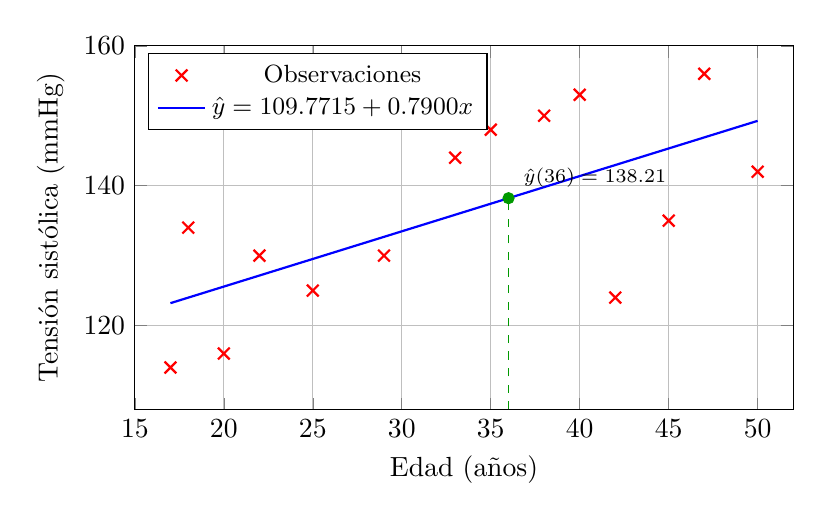
\begin{tikzpicture}
        \begin{axis}[width=.82\textwidth,height=6.2cm,xlabel={Edad (años)},ylabel={Tensión sistólica (mmHg)},xmin=15,xmax=52,ymin=108,ymax=160,grid=major,legend style={font=\small,at={(.02,.98)},anchor=north west}]
        \addplot[only marks,mark=x,mark size=3pt,red,thick] coordinates {(17,114)(18,134)(20,116)(22,130)(25,125)(29,130)(33,144)(35,148)(38,150)(40,153)(42,124)(45,135)(47,156)(50,142)};
        \addlegendentry{Observaciones}
        \addplot[blue,thick,domain=17:50,samples=2]{109.7715+0.7900*x};
        \addlegendentry{$\hat y=109.7715+0.7900x$}
        \addplot[green!60!black,dashed] coordinates {(36,108)(36,138.2115)};
        \addplot[only marks,mark=*,green!60!black] coordinates {(36,138.2115)};
        \node[font=\scriptsize,anchor=south west] at (axis cs:36.3,138.3) {$\hat y(36)=138.21$};
        \end{axis}
        \end{tikzpicture}
        \caption{Diagrama de dispersión y recta de regresión lineal para el ejemplo de Tensión Arterial vs. Edad de los pacientes.}
        \label{fig:tension}
    \end{figure}
 

\subsection{3. Deducción de las Ecuaciones Normales}
    Para encontrar los valores de $a$ y $b$ que hacen que la función de error $S(a, b)$ alcance su valor mínimo, aplicamos la herramienta por excelencia del análisis matemático: \textbf{derivadas parciales}. Derivamos respecto de $a$ y respecto de $b$, e igualamos a cero:
    \begin{align*}
        \frac{\partial S}{\partial a} &= 2 \sum_{i=1}^n \left[ y_i - (a + b \cdot x_i) \right] \cdot (-1) = 0 \\
        \frac{\partial S}{\partial b} &= 2 \sum_{i=1}^n \left[ y_i - (a + b \cdot x_i) \right] \cdot (-x_i) = 0
    \end{align*}
    Simplificando el factor 2 y distribuyendo las sumatorias, obtenemos el famoso \textbf{Sistema de Ecuaciones Normales (SEN)}:
    \begin{align*}
        n \cdot a + b \sum x_i &= \sum y_i \\
        a \sum x_i + b \sum x_i^2 &= \sum (x_i \cdot y_i)
    \end{align*}

    Este es un sistema lineal de dos ecuaciones con dos incógnitas ($a$ y $b$). Al resolverlo, ya sea por determinantes (Regla de Cramer) o mediante álgebra matricial inversa, se determinan los estimadores de mínimos cuadrados:
    \begin{equation}
        b = \frac{n \sum (x_i \cdot y_i) - \sum x_i \sum y_i}{n \sum x_i^2 - (\sum x_i)^2} \quad y \quad a = \bar{Y} - b \cdot \bar{X}
    \end{equation}
    Donde $\bar{X}$ y $\bar{Y}$ representan las medias muestrales de ambas variables.
 

\subsection{4. Resolución del Caso de Tensión Arterial}
    A partir de la muestra de $n = 14$ pacientes, realizamos los cálculos intermedios necesarios para armar el sistema:
    \begin{itemize}
        \item $\sum x_i = 461 \implies \bar{X} = 461/14 \approx 32.93$
        \item $\sum y_i = 1901 \implies \bar{Y} = 1901/14 \approx 135.79$
        \item $\sum x_i^2 = 16819$
        \item $\sum (x_i \cdot y_i) = 63892$
    \end{itemize}
    Calculamos la pendiente $b$:
    \[ b = \frac{14 \cdot (63892) - 461 \cdot 1901}{14 \cdot 16819 - 461^2} = \frac{894488 - 876361}{235466 - 212521} = \frac{18127}{22945} \approx \mathbf{0.7900} \]
    Calculamos la ordenada al origen $a$:
    \[ a = 135.7857 - 0.7899978 \cdot (32.9286) \approx \mathbf{109.7715} \]

    Por lo tanto, la ecuación predictora de mejor ajuste es:
    \[ \hat{y} = 109.7715 + 0.7900 \cdot x \]

    \textbf{Interpretación Intuitiva de los Parámetros:}
    \begin{itemize}
        \item $b = 0.7900$: Significa que, en promedio, por cada año adicional de edad de una persona, su tensión arterial sistólica aumenta aproximadamente en $0.79 \text{ mmHg}$.
        \item $a = 109.7715$: Es la ordenada al origen, una interpretación matemática del valor estimado de tensión para $x=0$ años. Queda fuera del rango observado ($17$ a $50$ años), por lo que no debe interpretarse como una medición real ni extrapolarse sin advertencia.
    \end{itemize}

    \textbf{Predicción para un Paciente de 36 años:}
    Sustituimos $x = 36$ en nuestra ecuación predictora:
    \[ \hat{y}(36) = 109.7715 + 0.7900 \cdot (36) \approx \mathbf{138.21 \text{ mmHg}} \]
 

\newpage
% -------------------------------------------------------------
% SUBSHEET: INFERENCIA EN REGRESIÓN
% -------------------------------------------------------------
\subsection{5. Inferencia Estadística en la Regresión (Pruebas e Intervalos)}
    \textbf{¿Cómo evaluamos si existe una relación lineal entre X e Y?} \label{ej:evaporacion_completo}
    Los coeficientes $a$ y $b$ que calculamos son estimadores muestrales de los verdaderos parámetros poblacionales $\alpha$ y $\beta$ (la recta real de la población es $Y = \alpha + \beta X + \epsilon$). Si la pendiente poblacional $\beta = 0$, la recta de regresión es horizontal y no hay relación lineal en este modelo. $X$ se utiliza como variable explicativa y $Y$ como variable respuesta; la regresión por sí sola no demuestra causalidad.

    Para abordar este tema, utilizaremos el \textbf{Ejemplo 2 (Gotitas de Combustible)} de tus fuentes.
    
    \textbf{Caso Práctico:} Se mide la velocidad del aire ($X$ en $\text{cm/s}$) y el coeficiente de evaporación de gotitas de combustible ($Y$ en $\text{mm}^2\text{/seg}$) en una turbina de propulsión ($n = 10$):
    \begin{table}[h!]
        \centering
        \caption{Datos de Velocidad del Aire y Coeficiente de Evaporación}
        \begin{tabular}{rcccccccccc}
            \toprule
            \textbf{Velocidad ($x_i$)} & 20 & 60 & 100 & 140 & 180 & 220 & 260 & 300 & 340 & 380 \\
            \textbf{Evaporación ($y_i$)} & 0.18 & 0.37 & 0.35 & 0.78 & 0.56 & 0.75 & 1.18 & 1.36 & 1.17 & 1.65 \\
            \bottomrule
        \end{tabular}
    \end{table}

    \begin{figure}[htbp]
        \centering
        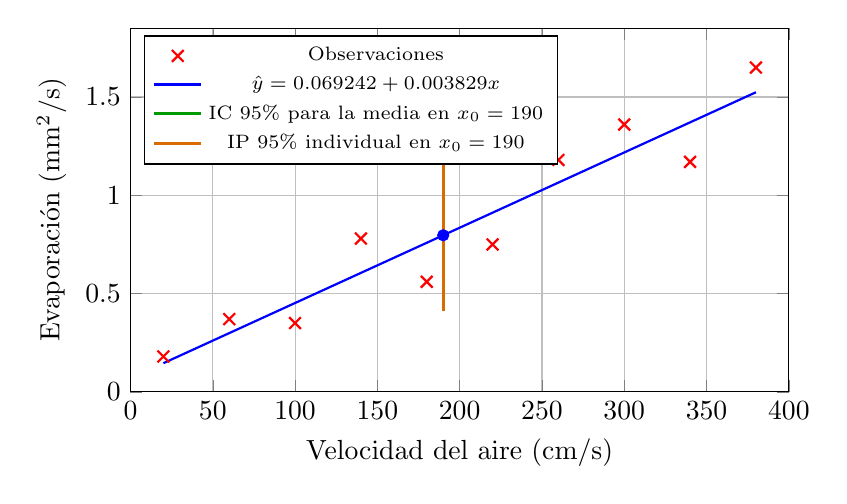
\begin{tikzpicture}
        \begin{axis}[width=.82\textwidth,height=6.2cm,xlabel={Velocidad del aire (cm/s)},ylabel={Evaporación (mm$^2$/s)},xmin=0,xmax=400,ymin=0,ymax=1.85,grid=major,legend style={font=\scriptsize,at={(.02,.98)},anchor=north west}]
        \addplot[only marks,mark=x,mark size=3pt,red,thick] coordinates {(20,.18)(60,.37)(100,.35)(140,.78)(180,.56)(220,.75)(260,1.18)(300,1.36)(340,1.17)(380,1.65)};
        \addlegendentry{Observaciones}
        \addplot[blue,thick,domain=20:380,samples=2]{0.069242+0.003829*x};
        \addlegendentry{$\hat y=0.069242+0.003829x$}
        \addplot[green!60!black,very thick] coordinates {(190,.6803)(190,.9131)};
        \addlegendentry{IC 95\% para la media en $x_0=190$}
        \addplot[orange!85!black,very thick] coordinates {(190,.4119)(190,1.1815)};
        \addlegendentry{IP 95\% individual en $x_0=190$}
        \addplot[only marks,mark=*,blue] coordinates {(190,.7967)};
        \end{axis}
        \end{tikzpicture}
        \caption{Recta de regresión e intervalos del 95\% en $x_0=190$: el intervalo de predicción individual es más ancho que el intervalo para la media.}
        \label{fig:evaporacion}
    \end{figure}

    \subsubsection*{Paso 1: Parámetros del Modelo y Notación Especial}
    Para simplificar las fórmulas de la inferencia, definimos tres sumas de cuadrados fundamentales:
    \begin{align}
        S_{xx} &= n \sum x_i^2 - \left(\sum x_i\right)^2 = 10 \cdot (532000) - 2000^2 = \mathbf{1.32 \times 10^6} \\
        S_{yy} &= n \sum y_i^2 - \left(\sum y_i\right)^2 = 10 \cdot (9.1097) - 8.35^2 = \mathbf{21.3745} \quad (\text{versión escalada}) \\
        S_{xy} &= n \sum (x_i \cdot y_i) - \sum x_i \sum y_i = 10 \cdot (2175.40) - 2000 \cdot 8.35 = \mathbf{5054.0} \quad (\text{versión escalada})
    \end{align}
    Si se utiliza la notación centrada, los valores equivalentes son $S_{xx,c}=S_{xx}/n=132000$, $S_{yy,c}=S_{yy}/n=2.13745$ y $S_{xy,c}=S_{xy}/n=505.4$. No deben mezclarse ambas versiones: la versión escalada se usa en las expresiones anteriores y la centrada en $b=S_{xy,c}/S_{xx,c}$.
    Calculamos la pendiente y ordenada al origen muestrales:
    \begin{align*}
        b &= \frac{S_{xy}}{S_{xx}} = \frac{5054.0}{1320000} \approx \mathbf{0.003829} \quad (\text{o } 3.829 \times 10^{-3}) \\
        a &= \bar{Y} - b \bar{X} = 0.835 - 0.00382879 \cdot (200) = \mathbf{0.069242}
    \end{align*}

    \subsubsection*{Paso 2: Estimación de la Varianza del Error ($\sigma^2$)}
    La varianza de la perturbación aleatoria ($\sigma^2$) mide la dispersión física de los puntos reales alrededor de la recta verdadera de la población. La estimamos mediante la \textbf{varianza residual muestral} $s_e^2$, con $n-2$ grados de libertad; su raíz $s_e$ es el error estándar de estimación:
    \begin{equation}
        s_e^2 = \frac{S_{xx} \cdot S_{yy} - S_{xy}^2}{n(n-2) \cdot S_{xx}} = \frac{1320000 \cdot 21.3745 - 5054^2}{10 \cdot 8 \cdot 1320000} \approx \mathbf{0.025298} \implies s_e \approx \mathbf{0.159052}
    \end{equation}

    \subsubsection*{Paso 3: Prueba de Hipótesis para la Pendiente ($\beta = 0$)}
    Queremos contrastar si existe una relación lineal real o si el valor de la pendiente $b$ se debe meramente al azar:
    \begin{align*}
        H_0&: \beta = 0 \quad (\text{No hay relación lineal, la recta es horizontal}) \\
        H_1&: \beta \neq 0 \quad (\text{Existe relación lineal significativa, prueba bilateral})
    \end{align*}
    Utilizamos un nivel de significación de $\alpha = 0.05$. Para $n-2 = 8$ grados de libertad, el valor crítico en la distribución $t$ de Student de dos colas es:
    \[ t_{\text{crit}} = \pm t_{0.025, 8} = \mathbf{\pm 2.306} \]

    Calculamos nuestro estadístico de prueba estandarizado $t_{\text{calc}}$:
    \begin{equation}
        t_{\text{calc}} = \frac{b - \beta_0}{s_e} \cdot \sqrt{\frac{S_{xx}}{n}} = \frac{0.003829 - 0}{0.159052} \cdot \sqrt{\frac{1320000}{10}} = 0.024074 \cdot (363.318) = \mathbf{8.7460}
    \end{equation}

    \textbf{Decisión:} Como $|t_{\text{calc}}| = 8.7460 > 2.306$, se rechaza la hipótesis nula $H_0$. Existe evidencia de una relación lineal estadísticamente significativa entre la velocidad del aire y la evaporación del combustible en la turbina. Esta conclusión no demuestra causalidad.

    \subsubsection*{Paso 4: Intervalo de Confianza para la Media de Y dada una velocidad fija ($x_0 = 190$)}
    Si fijamos una velocidad del aire de $x_0 = 190 \text{ cm/s}$, ¿cuál es el valor medio esperado del coeficiente de evaporación?
    El estimador puntual es:
    \[ \hat{y}(190) = a + b \cdot 190 = 0.069242 + 0.003829 \cdot 190 = \mathbf{0.7967 \text{ mm}^2\text{/seg}} \]
    El error máximo de estimación para la media poblacional $\mu_Y$ con un 95\% de confianza es:
    \[ E = t_{\alpha/2, n-2} \cdot s_e \cdot \sqrt{\frac{1}{n} + \frac{n(x_0 - \bar{X})^2}{S_{xx}}} \]
    Sustituyendo los valores numéricos:
    \[ E = 2.306 \cdot 0.159052 \cdot \sqrt{\frac{1}{10} + \frac{10 \cdot (190 - 200)^2}{1320000}} = 0.36677 \cdot \sqrt{0.100757} = \mathbf{0.1164} \]
    Por lo tanto, el intervalo de confianza del 95\% para el valor medio es:
    \[ 0.7967 \pm 0.1164 \implies \mathbf{[0.6803 \, , \, 0.9131] \text{ mm}^2\text{/seg}} \]

    \subsubsection*{Paso 5: Intervalo de Predicción para una Observación Futura Individual en $x_0 = 190$}
    ¿Qué pasa si en lugar de predecir la media de muchos ensayos queremos anticipar el resultado de \textbf{un único ensayo futuro}? La incertidumbre será mucho mayor, puesto que a la variabilidad de estimar la recta se le suma la dispersión física natural del proceso ($\sigma^2$).
    La fórmula del error máximo de predicción individual agrega un "$1$" dentro de la raíz:
    \[ E_{\text{pred}} = t_{\alpha/2, n-2} \cdot s_e \cdot \sqrt{1 + \frac{1}{n} + \frac{n(x_0 - \bar{X})^2}{S_{xx}}} \]
    Sustituyendo los valores:
    \[ E_{\text{pred}} = 2.306 \cdot 0.159052 \cdot \sqrt{1.100757} = 0.36677 \cdot (1.04917) = \mathbf{0.3848} \]
    Por lo tanto, el intervalo de predicción individual del 95\% es:
    \[ 0.7967 \pm 0.3848 \implies \mathbf{[0.4119 \, , \, 1.1815] \text{ mm}^2\text{/seg}} \]
    
    Como se aprecia, este intervalo es considerablemente más ancho que el del valor medio.
 

\subsection{6. Guion oral breve para exponer la Regresión Simple}
    \begin{guion}
        \textbf{Frase de Inicio:} "Estimado tribunal, voy a exponer el tema de Regresión Lineal Simple detallando cómo construimos un modelo que no solo asocia variables, sino que nos permite hacer predicciones confiables bajo incertidumbre..."
        
        \textbf{Desarrollo Verbal:} "Para entender este concepto, consideremos el caso de la turbina donde medimos la velocidad del aire y la evaporación del combustible. Si graficamos los datos crudos, advertimos que no están perfectamente alineados. El método de los mínimos cuadrados nos permite encontrar la única recta que minimiza de forma conjunta el cuadrado de las distancias verticales de las observaciones a la recta. Al derivar parcialmente esta suma de errores e igualar a cero, deducimos el sistema de ecuaciones normales que nos entrega la ordenada $a=0.069$ y la pendiente $b=0.0038$. 
        
        Para validar si esta pendiente es real, sometemos a prueba la hipótesis nula de que $\beta=0$. Nuestro estadístico calculado $t$ arroja un valor de $8.75$, el cual supera holgadamente la frontera crítica de Student de $2.306$. Por lo tanto, rechazamos la hipótesis de que no hay relación lineal y afirmamos que existe evidencia de una relación lineal estadísticamente significativa. La regresión por sí sola no demuestra causalidad.
        
        Finalmente, al predecir para una velocidad de $190 \text{ cm/s}$, obtenemos una evaporación puntual de $0.80 \text{ mm}^2\text{/s}$. Es crucial destacar ante el tribunal la diferencia entre el intervalo para el valor promedio y el intervalo para una observación futura individual. El de predicción individual siempre será más ancho —en este caso, varía de $0.41$ a $1.18$— porque debe absorber tanto el error de estimación de la recta como la variabilidad aleatoria intrínseca del proceso físico."
        
        \textbf{Frase de Cierre:} "...con esto concluyo la exposición de regresión lineal, demostrando que la inferencia estadística es la herramienta fundamental para cuantificar el error y tomar decisiones ingenieriles con sustento probabilístico."
    \end{guion}
 

\clearpage
% -------------------------------------------------------------
% SECCIÓN 4: REGRESIÓN CURVILÍNEA (TEMA A-2)
% -------------------------------------------------------------
\section{Tema A-2: Regresión Curvilínea y Linealización de Datos}

\begin{ruta}
\textbf{Elegir por forma y mecanismo:} exponencial para cambios multiplicativos; potencial para leyes de escala; recíproco para una relación con asíntota. En los tres casos se ajusta una recta en la escala transformada, se revisan sus residuos y se retransforma antes de interpretar o predecir.
\end{ruta}

¿Qué ocurre si al realizar el diagrama de dispersión inicial advertimos que los datos no siguen en absoluto una trayectoria recta? Si intentáramos ajustar una línea recta de todos modos por mínimos cuadrados, la matemática nos entregaría coeficientes, pero el modelo realizaría pésimas predicciones porque no respeta la naturaleza del fenómeno (ver Figura \ref{fig:exponencial}).

Ante esto, contamos con dos opciones: desarrollar complejos algoritmos de regresión no lineal, o aplicar una \textbf{transformación matemática específica a los datos originales} para que se comporten de forma lineal, permitiendo aplicar el método clásico de mínimos cuadrados que ya dominamos. En el modelo exponencial se transforma $Y$ (por ejemplo, $\log(Y)$) y se mantiene $X$; en el potencial se transforman ambas variables ($\log(X)$ y $\log(Y)$); en el recíproco se transforma $Y$ mediante $1/Y$. Luego debe realizarse la retransformación a la escala original. Esta última es la alternativa más sencilla dentro de las fuentes.

Estudiaremos tres modelos de transformación curvilínea que son clásicos de examen:

\subsection{1. Modelo Exponencial ($y = \alpha \cdot \beta^x$)}
    \textbf{Caso Práctico:} Un fabricante de neumáticos estudia el desgaste de sus llantas radiales registrando el porcentaje útil de goma ($Y$) luego de recorrer ciertas millas de prueba ($X$, en miles de millas):
    \begin{table}[h!]
        \centering
        \caption{Porcentaje Útil de Neumáticos según Millas Recorridas}
        \begin{tabular}{rcccccccc}
            \toprule
            \textbf{Miles de Millas ($x_i$)} & 1 & 2 & 5 & 10 & 20 & 30 & 40 & 50 \\
            \textbf{Porcentaje útil ($y_i$)} & 98.2 & 91.7 & 81.3 & 64.0 & 36.4 & 32.6 & 17.1 & 11.3 \\
            \bottomrule
        \end{tabular}
    \end{table}

    \textbf{¿Qué buscamos responder?}
    \begin{itemize}
        \item ¿Es razonable suponer que el desgaste del neumático es proporcional a su uso (decae exponencialmente)?
        \item ¿Qué porcentaje de neumáticos del fabricante durarán menos de 25,000 millas (predicción para $x = 25$)?
    \end{itemize}

    \subsubsection*{Deducción de la Linealización Exponencial}
    Planteamos la ecuación exponencial original de la población:
    \[ y = \alpha \cdot \beta^x \]
    Para linealizarla, aplicamos \textbf{logaritmo base 10} a ambos miembros de la ecuación:
    \[ \log_{10}(y) = \log_{10}(\alpha \cdot \beta^x) \]
    Por propiedades de los logaritmos, el logaritmo de un producto es la suma de los logaritmos, y el exponente de la variable baja multiplicando:
    \begin{equation}
        \log_{10}(y) = \log_{10}(\alpha) + x \cdot \log_{10}(\beta)
    \end{equation}
    Si definimos las variables transformadas:
    \[ y^* = \log_{10}(y), \quad a = \log_{10}(\alpha), \quad b = \log_{10}(\beta) \]
    Nuestra ecuación predictora se transforma en una recta perfecta:
    \[ y^* = a + b \cdot x \]

    \begin{figure}[htbp]
        \centering
        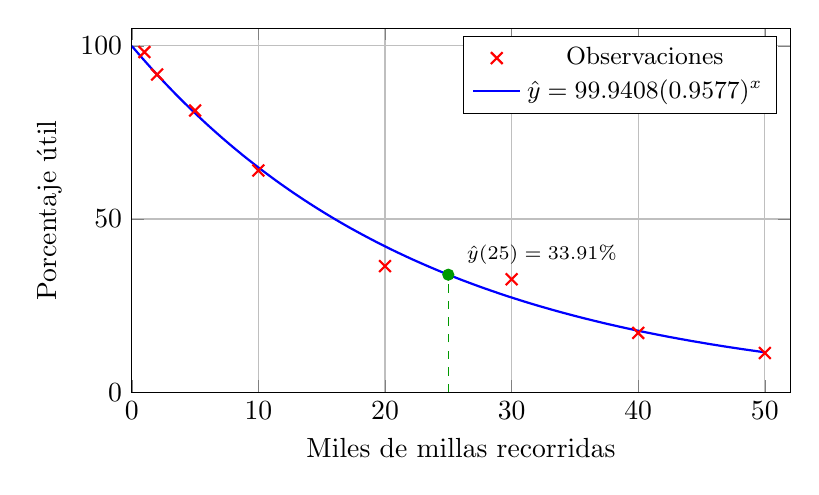
\begin{tikzpicture}
        \begin{axis}[width=.82\textwidth,height=6.2cm,xlabel={Miles de millas recorridas},ylabel={Porcentaje útil},xmin=0,xmax=52,ymin=0,ymax=105,grid=major,legend style={font=\small,at={(.98,.98)},anchor=north east}]
        \addplot[only marks,mark=x,mark size=3pt,red,thick] coordinates {(1,98.2)(2,91.7)(5,81.3)(10,64)(20,36.4)(30,32.6)(40,17.1)(50,11.3)};
        \addlegendentry{Observaciones}
        \addplot[blue,thick,domain=0:50,samples=120]{99.9408*0.9577^x};
        \addlegendentry{$\hat y=99.9408(0.9577)^x$}
        \addplot[green!60!black,dashed] coordinates {(25,0)(25,33.91)};
        \addplot[only marks,mark=*,green!60!black] coordinates {(25,33.91)};
        \node[font=\scriptsize,anchor=south west] at (axis cs:25.7,34) {$\hat y(25)=33.91\%$};
        \end{axis}
        \end{tikzpicture}
        \caption{Ajuste Curvilíneo Exponencial para los datos del porcentaje útil de llantas radiales.}
        \label{fig:exponencial}
    \end{figure}

    \subsubsection*{Resolución Numérica Paso a Paso}
    Calculamos el logaritmo base 10 de cada valor de nuestra variable explicada $Y$:
    \[ \log_{10}(y) = [1.9921, \, 1.9624, \, 1.9101, \, 1.8062, \, 1.5611, \, 1.5132, \, 1.2330, \, 1.0531] \]
    Ahora, resolvemos el ajuste lineal clásico utilizando las parejas $[x_i, y^*_i]$. Nuestra muestra tiene $n = 8$:
    \begin{itemize}
        \item $\sum x_i = 158$
        \item $\sum y^*_i = 13.0311$
        \item $\sum x_i^2 = 5530$
        \item $\sum (x_i \cdot y^*_i) = 212.1214$
    \end{itemize}
    Calculamos los parámetros de la recta transformada:
    \begin{align*}
        b = \frac{8 \cdot (212.1214) - 158 \cdot (13.0311)}{8 \cdot 5530 - 158^2} \approx \frac{-361.93}{19276} \approx \mathbf{-0.0188} \\
        a = \bar{Y}^* - b \bar{X} = 1.6289 - (-0.0188) \cdot (19.75) \approx \mathbf{1.9997}
    \end{align*}

    \subsubsection*{Retransformación a la Forma Original (¡La clave de examen!)}
    \begin{importante}
        \textbf{¡Atención! Error clásico de examen de último minuto:} Muchos estudiantes cometen el grave error de escribir la función final directamente con los valores de la recta transformada ($a$ y $b$). Recuerda que para realizar la predicción en la escala real de las variables, debes \textbf{deshacer la transformación} aplicando la operación inversa (exponenciación base 10):
        \begin{align}
            \alpha &= 10^a = 10^{1.9997} \approx \mathbf{99.9408} \\
            \beta &= 10^b = 10^{-0.0188} \approx \mathbf{0.9577}
        \end{align}
    \end{importante}
    La verdadera función predictora en la escala original del problema físico es:
    \[ y = 99.9408 \cdot (0.9577)^x \]

    \subsubsection*{Predicción para x = 25 (25,000 millas)}
    Sustituimos $x = 25$ en nuestra función original retransformada:
    \[ y(25) = 99.9408 \cdot (0.9577)^{25} = 99.9408 \cdot 0.3393 = \mathbf{33.91\%} \]
    Esto significa que se estima que el 33.91\% de la goma útil del neumático quedará sana tras recorrer 25,000 millas.
 

\newpage
% -------------------------------------------------------------
% MODELO POTENCIAL Y RECÍPROCO
% -------------------------------------------------------------
\subsection{2. Modelo Potencial ($y = \alpha \cdot x^\beta$)}
    Cuando los datos se distribuyen de forma que en un papel de escala doble logarítmica se alinean como una recta, se utiliza la ley de potencia.
    
    Planteamos el modelo:
    \[ y = \alpha \cdot x^\beta \]
    Aplicamos logaritmos base 10 a ambos miembros de la ecuación:
    \begin{equation}
        \log_{10}(y) = \log_{10}(\alpha) + \beta \cdot \log_{10}(x)
    \end{equation}
    Definimos variables transformadas para linealizar:
    \[ y^* = \log_{10}(y), \quad x^* = \log_{10}(x), \quad a = \log_{10}(\alpha), \quad B = \beta \]
    La ecuación predictora resultante es lineal en ambas escalas:
    \[ y^* = a + B \cdot x^* \]
    
    En este caso, debemos calcular las sumatorias aplicando logaritmos tanto a la variable $X$ como a la variable $Y$ antes de resolver por mínimos cuadrados. Una vez obtenidos $a$ y $b$ de la recta transformada, la retransformación es:
    \[ \alpha = 10^a \quad \text{y} \quad \beta = b \]

    \begin{figure}[htbp]
        \centering
        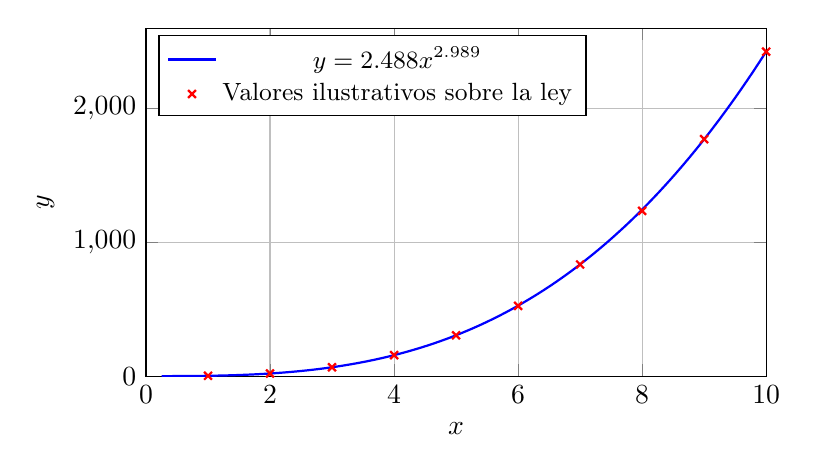
\begin{tikzpicture}
        \begin{axis}[width=.78\textwidth,height=6cm,xlabel={$x$},ylabel={$y$},xmin=0,xmax=10,ymin=0,ymax=2600,grid=major,legend style={font=\small,at={(.02,.98)},anchor=north west}]
        \addplot[blue,thick,domain=.25:10,samples=120]{2.488*x^2.989};
        \addlegendentry{$y=2.488x^{2.989}$}
        \addplot[only marks,mark=x,red,thick] coordinates {(1,2.5)(2,19.7)(3,66.4)(4,157)(5,305)(6,525)(7,834)(8,1235)(9,1771)(10,2425)};
        \addlegendentry{Valores ilustrativos sobre la ley}
        \end{axis}
        \end{tikzpicture}
        \caption{Forma de una función potencial. Es un ejemplo conceptual: la comprobación se realiza verificando linealidad en el gráfico de $\log y$ frente a $\log x$.}
        \label{fig:potencial}
    \end{figure}
 

\subsection{3. Modelo Recíproco ($y = \frac{1}{\alpha + \beta \cdot x}$)}
    Este modelo es de gran aplicación práctica para describir curvas de saturación, procesos de decaimiento asintótico o relaciones de velocidad/rendimiento que decrecen rápidamente sin volverse negativas (ver Figura \ref{fig:reciproca}).

    Planteamos el modelo recíproco:
    \[ y = \frac{1}{\alpha + \beta \cdot x} \]
    Para linealizar, simplemente aplicamos la inversa multiplicativa a ambos lados de la igualdad:
    \begin{equation}
        \frac{1}{y} = \alpha + \beta \cdot x
    \end{equation}
    Definiendo la variable transformada $y^* = 1/y$, la relación se vuelve lineal:
    \[ y^* = a + b \cdot x \]
    Donde los estimadores directos se mantienen sin alterar:
    \[ \alpha = a \quad \text{y} \quad \beta = b \]

    \begin{figure}[htbp]
        \centering
        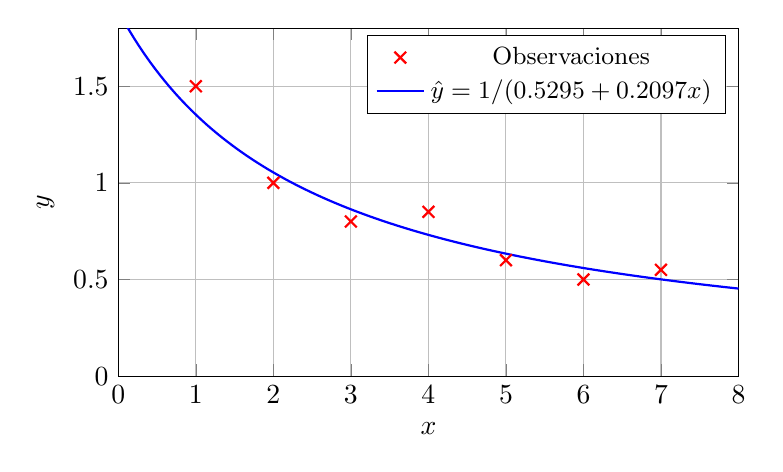
\begin{tikzpicture}
        \begin{axis}[width=.78\textwidth,height=6cm,xlabel={$x$},ylabel={$y$},xmin=0,xmax=8,ymin=0,ymax=1.8,grid=major,legend style={font=\small,at={(.98,.98)},anchor=north east}]
        \addplot[only marks,mark=x,mark size=3pt,red,thick] coordinates {(1,1.5)(2,1)(3,.8)(4,.85)(5,.6)(6,.5)(7,.55)};
        \addlegendentry{Observaciones}
        \addplot[blue,thick,domain=0:8,samples=120]{1/(0.5295+0.2097*x)};
        \addlegendentry{$\hat y=1/(0.5295+0.2097x)$}
        \end{axis}
        \end{tikzpicture}
        \caption{Ajuste Curvilíneo Recíproco para el decaimiento asintótico de las observaciones experimentales.}
        \label{fig:reciproca}
    \end{figure}

    \subsubsection*{Ejercicio Resuelto Integrador del Modelo Recíproco}
    \textbf{Caso Práctico:} Se dispone del siguiente conjunto de datos experimentales donde $X$ es la variable controlada e $Y$ es la respuesta física observada:
    \begin{table}[h!]
        \centering
        \begin{tabular}{rccccccc}
            \toprule
            \textbf{$x_i$} & 1 & 2 & 3 & 4 & 5 & 6 & 7 \\
            \textbf{$y_i$} & 1.5 & 1.0 & 0.8 & 0.85 & 0.6 & 0.5 & 0.55 \\
            \bottomrule
        \end{tabular}
    \end{table}

    Realizamos la transformación recíproca de la variable explicada, calculando $y^*_i = 1/y_i$ para cada una de las $n = 7$ observaciones:
    \[ y^* = [0.6667, \, 1.0000, \, 1.2500, \, 1.1765, \, 1.6667, \, 2.0000, \, 1.8182] \]
    Calculamos las sumas intermedias requeridas:
    \begin{itemize}
        \item $\sum x_i = 28$
        \item $\sum y^*_i = 9.578$
        \item $\sum x_i^2 = 140$
        \item $\sum (x_i \cdot y^*_i) = 44.183$
    \end{itemize}
    Utilizamos el Sistema de Ecuaciones Normales por determinantes:
    \[ \Delta = \begin{vmatrix} n & \sum x_i \\ \sum x_i & \sum x_i^2 \end{vmatrix} = \begin{vmatrix} 7 & 28 \\ 28 & 140 \end{vmatrix} = 7 \cdot 140 - 28^2 = 980 - 784 = \mathbf{196} \]
    Calculamos el numerador para $a$:
    \begin{align*}
    \Delta_a
      &= \begin{vmatrix} \sum y^*_i & \sum x_i \\ \sum (x_i y^*_i) & \sum x_i^2 \end{vmatrix}
       = \begin{vmatrix} 9.578 & 28 \\ 44.183 & 140 \end{vmatrix} \\
      &= 9.578 \cdot 140 - 44.183 \cdot 28
       = 1340.92 - 1237.124 = \mathbf{103.796}
    \end{align*}
    \[ a = \frac{\Delta_a}{\Delta} = \frac{103.796}{196} \approx \mathbf{0.5295} \]
    Calculamos el numerador para $b$:
    \[ \Delta_b = \begin{vmatrix} n & \sum y^*_i \\ \sum x_i & \sum (x_i y^*_i) \end{vmatrix} = \begin{vmatrix} 7 & 9.578 \\ 28 & 44.183 \end{vmatrix} = 7 \cdot 44.183 - 28 \cdot 9.578 = 309.281 - 268.184 = \mathbf{41.097} \]
    \[ b = \frac{\Delta_b}{\Delta} = \frac{41.097}{196} \approx \mathbf{0.2097} \]

    \textbf{Función Predictora Final:}
    Retransformamos de manera directa, dado que $\alpha = a$ y $\beta = b$:
    \[ y = \frac{1}{0.5295 + 0.2097 \cdot x} \]
 

\clearpage
% -------------------------------------------------------------
% SECCIÓN 5: AJUSTE POLINÓMICO (TEMA B-1)
% -------------------------------------------------------------
\section{Tema B-1: Ajuste Polinómico y Selección de Grado}

\begin{ruta}
\textbf{Cuándo usar:} existe curvatura sin una familia física simple. Ajustar grados sucesivos con $p<n-1$, comparar $s^2_{res}=\mathrm{SCE}/(n-p-1)$ y volver a revisar residuos. Detenerse en el menor grado que produzca una mejora sustancial para evitar sobreajuste.
\end{ruta}

¿Qué ocurre si la relación entre $X$ e $Y$ es tan compleja, oscilatoria o errática que no se alinea con ninguna transformación simple como el logaritmo o la recíproca?

Cuando no se conoce una forma funcional simple, puede utilizarse un polinomio como aproximación empírica de la relación observada. El grado debe elegirse equilibrando capacidad de ajuste y riesgo de sobreajuste.

Un polinomio de grado $p$ tiene la siguiente ecuación predictora:
\begin{equation}
    y = \beta_0 + \beta_1 \cdot x + \beta_2 \cdot x^2 + \beta_3 \cdot x^3 + \dots + \beta_p \cdot x^p
\end{equation}

\subsection{1. Deducción del Sistema de Ecuaciones Normales}
    Para estimar los $p+1$ coeficientes ($\beta_j$) del polinomio, aplicamos nuevamente el criterio de mínimos cuadrados, minimizando la Suma de Cuadrados del Error (SCE):
    \[ S(\beta_0, \beta_1, \dots, \beta_p) = \sum_{i=1}^n e_i^2 = \sum_{i=1}^n \left[ y_i - (\beta_0 + \beta_1 \cdot x_i + \beta_2 \cdot x_i^2 + \dots + \beta_p \cdot x_i^p) \right]^2 \]
    Derivamos parcialmente respecto de cada uno de los $p+1$ coeficientes e igualamos a cero, obteniendo un conjunto de ecuaciones lineales que conforman un sistema perfectamente estructurado. Por ejemplo, para un polinomio de grado 2 (parábola, ver Figura \ref{fig:secado}), el sistema de ecuaciones normales resulta:
    \begin{align*}
        n \cdot b_0 + b_1 \sum x_i + b_2 \sum x_i^2 &= \sum y_i \\
        b_0 \sum x_i + b_1 \sum x_i^2 + b_2 \sum x_i^3 &= \sum (x_i \cdot y_i) \\
        b_0 \sum x_i^2 + b_1 \sum x_i^3 + b_2 \sum x_i^4 &= \sum (x_i^2 \cdot y_i)
    \end{align*}

    Este sistema se puede compactar de forma elegante en una matriz simétrica de tamaño $3 \times 3$, que resolvemos de forma eficiente utilizando determinantes o álgebra computacional.

    \begin{figure}[htbp]
        \centering
        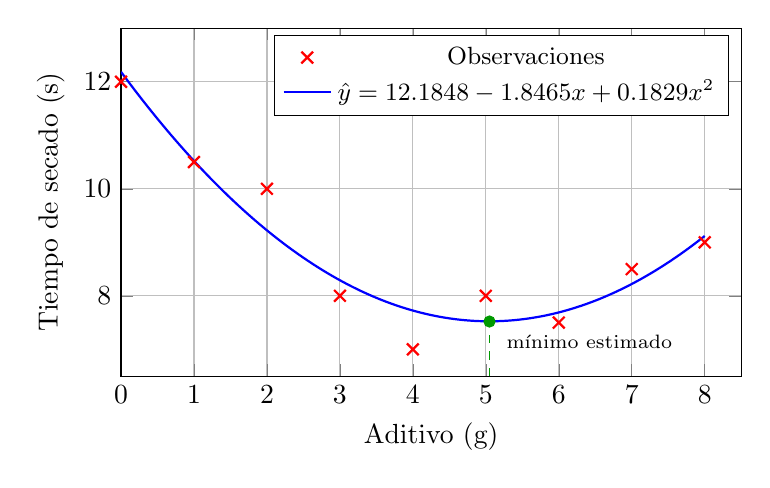
\begin{tikzpicture}
        \begin{axis}[width=.78\textwidth,height=6cm,xlabel={Aditivo (g)},ylabel={Tiempo de secado (s)},xmin=0,xmax=8.5,ymin=6.5,ymax=13,grid=major,legend style={font=\small,at={(.98,.98)},anchor=north east}]
        \addplot[only marks,mark=x,mark size=3pt,red,thick] coordinates {(0,12)(1,10.5)(2,10)(3,8)(4,7)(5,8)(6,7.5)(7,8.5)(8,9)};
        \addlegendentry{Observaciones}
        \addplot[blue,thick,domain=0:8,samples=120]{12.1848-1.8465*x+0.1829*x^2};
        \addlegendentry{$\hat y=12.1848-1.8465x+0.1829x^2$}
        \addplot[green!60!black,dashed] coordinates {(5.05,6.5)(5.05,7.52)};
        \addplot[only marks,mark=*,green!60!black] coordinates {(5.05,7.52)};
        \node[font=\scriptsize,anchor=north west] at (axis cs:5.15,7.45) {mínimo estimado};
        \end{axis}
        \end{tikzpicture}
        \caption{Ajuste Polinómico de Segundo Grado para el tiempo de secado en segundos según los gramos de aditivo utilizados.}
        \label{fig:secado}
    \end{figure}
 

\subsection{2. Ejemplo Práctico de Ajuste Parabólico (Tiempo de Secado)}
    \textbf{Caso Práctico:} En un proceso de fabricación de barniz, se desea estudiar la relación entre la cantidad de sustancia aditiva y el tiempo de secado. Se ensayan 9 combinaciones en el laboratorio:
    \begin{table}[h!]
        \centering
        \caption{Tiempo de Secado según Cantidad de Aditivo}
        \begin{tabular}{rccccccccc}
            \toprule
            \textbf{Aditivo gr. ($x_i$)} & 0 & 1 & 2 & 3 & 4 & 5 & 6 & 7 & 8 \\
            \textbf{Secado seg. ($y_i$)} & 12.0 & 10.5 & 10.0 & 8.0 & 7.0 & 8.0 & 7.5 & 8.5 & 9.0 \\
            \bottomrule
        \end{tabular}
    \end{table}

    \textbf{¿Qué buscamos responder?}
    \begin{itemize}
        \item ¿Es adecuada una relación parabólica?
        \item ¿Cuál es la cantidad óptima de aditivo para lograr el menor tiempo de secado?
    \end{itemize}

    \subsubsection*{Resolución Desarrollada de la Parábola de Mínimos Cuadrados}
    Nuestra muestra consta de $n = 9$ observaciones continuas de aditivo ($X$) y tiempo ($Y$). Realizamos los cálculos de las sumas:
    \begin{itemize}
        \item $\sum x_i = 36$
        \item $\sum y_i = 80.5$
        \item $\sum x_i^2 = 204$
        \item $\sum x_i^3 = 1296$
        \item $\sum x_i^4 = 8772$
        \item $\sum (x_i \cdot y_i) = 299.0$
        \item $\sum (x_i^2 \cdot y_i) = 1697.0$
    \end{itemize}
    Sustituyendo estas sumas en el sistema simétrico de ecuaciones normales, obtenemos:
    \[ \begin{bmatrix} 9 & 36 & 204 \\ 36 & 204 & 1296 \\ 204 & 1296 & 8772 \end{bmatrix} \begin{bmatrix} b_0 \\ b_1 \\ b_2 \end{bmatrix} = \begin{bmatrix} 80.5 \\ 299.0 \\ 1697.0 \end{bmatrix} \]
    Resolviendo este sistema mediante el método inverso o por determinantes, se obtienen los coeficientes del polinomio:
    \begin{equation}
        b_0 = \mathbf{12.1848}, \quad b_1 = \mathbf{-1.8465}, \quad b_2 = \mathbf{0.1829}
    \end{equation}
    Por lo tanto, la parábola predictora óptima es:
    \[ \hat{y} = 12.1848 - 1.8465 \cdot x + 0.1829 \cdot x^2 \]

    \subsubsection*{Optimización e Interpretación Contextual}
    Dado que el coeficiente cuadrático $b_2 = 0.1829$ es positivo, la parábola se abre hacia arriba (cóncava hacia arriba), lo que confirma la existencia de un \textbf{tiempo de secado mínimo}. Para hallar esta dosis óptima de aditivo, derivamos la ecuación predictora respecto a $X$ e igualamos a cero:
    \[ \frac{d\hat{y}}{dx} = b_1 + 2 \cdot b_2 \cdot x = -1.8465 + 2 \cdot (0.1829) \cdot x = 0 \]
    \[ x_{\text{óptimo}} = \frac{-b_1}{2 \cdot b_2} = \frac{1.8465}{2 \cdot 0.1829} = \mathbf{5.05 \text{ gramos de aditivo}} \]
    El tiempo mínimo estimado que se alcanzará con esta dosis es de:
    \[ \hat{y}(5.05) = 12.1848 - 1.8465 \cdot (5.05) + 0.1829 \cdot (5.05)^2 \approx \mathbf{7.52 \text{ segundos}} \]
 

\newpage
% -------------------------------------------------------------
% SECCIÓN: SELECCIÓN DEL GRADO POR VARIANZA RESIDUAL
% -------------------------------------------------------------
\subsection{3. El Criterio Riguroso de la Varianza Residual}
    \textbf{¿Cómo decidimos hasta qué grado del polinomio es conveniente ajustar?}
    A primera vista, se podría pensar que cuanto mayor sea el grado del polinomio, mejor será el modelo, puesto que la curva pasará más cerca de todos los puntos muestrales. De hecho, si tenemos $n$ puntos y ajustamos un polinomio de grado $p = n - 1$, la curva pasará exactamente por todos y cada uno de los puntos, anulando por completo la Suma de Cuadrados de Error (SCE $= 0$).
    
    Sin embargo, esto constituye un grave error llamado \textbf{Sobreajuste (Overfitting)}. Al obligar a la función a pasar por todos los puntos, el modelo capturará el ruido aleatorio del muestreo en lugar de la verdadera tendencia física subyacente. El resultado será una curva con oscilaciones salvajes y absurdas que realizará pésimos pronósticos ante nuevos datos.

    Para evitar este escollo de forma rigurosa en el examen, utilizamos la \textbf{Varianza Residual ($\sigma^2_{\text{res}}$)}:
    \begin{equation}
        \sigma^2_{\text{res}} = \frac{\sum_{i=1}^n (y_i - \hat{y}_i)^2}{n - (p + 1)}
    \end{equation}
    Donde:
    \begin{itemize}
        \item $n$ es la cantidad de puntos de la muestra.
        \item $p$ es el grado del polinomio (por lo que $p+1$ es la cantidad de coeficientes estimados).
        \item $n - p - 1$ son los \textbf{grados de libertad} del modelo.
    \end{itemize}

    \textbf{El procedimiento utilizado por la cátedra:}
    Alineado con lo explicado por tus profesores Peretti y Guarnier, se comienza ajustando una línea recta (grado $1$), luego una parábola (grado $2$), luego un polinomio cúbico (grado $3$), y así sucesivamente, calculando la varianza residual para cada modelo.
    
    A medida que aumentamos el grado, el numerador (SCE) disminuye, pero también lo hace el denominador (grados de libertad). Por lo tanto, llegará un punto donde la varianza residual deje de bajar significativamente o incluso empiece a subir. Según el criterio utilizado por la cátedra, el grado se selecciona donde se observe la mayor caída ("el salto decreciente más significativo") de la varianza residual. No se presenta este salto como un criterio estadístico universal; continuar aumentando el grado puede ser innecesario y aumentar el riesgo de sobreajuste.

    \subsubsection*{El Caso Práctico de la Varianza Residual (10 puntos)}
    Consideremos la muestra de $n = 10$ puntos de tus fuentes (ver Figura \ref{fig:residual}):
    \begin{table}[h!]
        \centering
        \begin{tabular}{rcccccccccc}
            \toprule
            \textbf{$x_i$} & 0.5 & 1.5 & 2.5 & 5.5 & 6.5 & 9.5 & 10.5 & 12.5 & 14.5 & 15.5 \\
            \textbf{$y_i$} & 3.0 & 7.0 & 12.5 & 14.5 & 16.0 & 14.5 & 16.0 & 16.0 & 21.0 & 23.0 \\
            \bottomrule
        \end{tabular}
    \end{table}

    \begin{figure}[htbp]
        \centering
        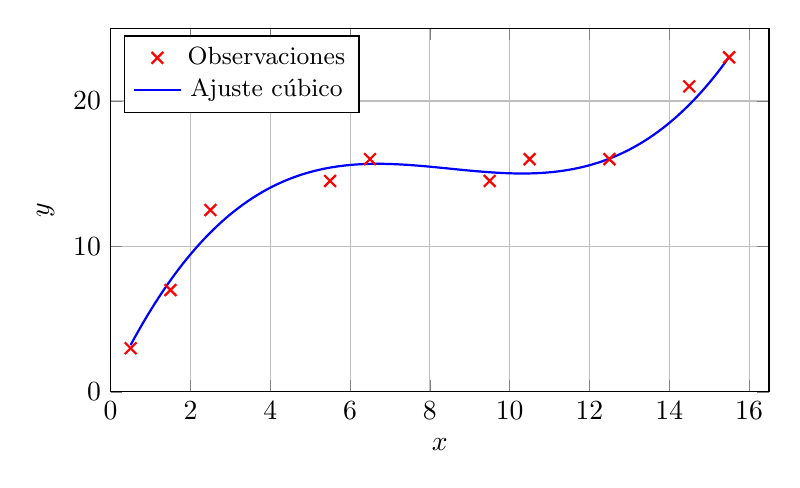
\begin{tikzpicture}
        \begin{axis}[width=.82\textwidth,height=6.2cm,xlabel={$x$},ylabel={$y$},xmin=0,xmax=16.5,ymin=0,ymax=25,grid=major,legend style={font=\small,at={(.02,.98)},anchor=north west}]
        \addplot[only marks,mark=x,mark size=3pt,red,thick] coordinates {(.5,3)(1.5,7)(2.5,12.5)(5.5,14.5)(6.5,16)(9.5,14.5)(10.5,16)(12.5,16)(14.5,21)(15.5,23)};
        \addlegendentry{Observaciones}
        \addplot[blue,thick,domain=.5:15.5,samples=150]{0.497+5.793*x-0.714*x^2+0.028*x^3};
        \addlegendentry{Ajuste cúbico}
        \end{axis}
        \end{tikzpicture}
        \caption{Ajuste cúbico asociado a la caída principal de la varianza residual. La tabla posterior compara los grados candidatos.}
        \label{fig:residual}
    \end{figure}

    Evaluamos el ajuste polinómico sucesivo, calculando los resultados exactos que se consolidan en la siguiente tabla de examen:
    \begin{table}[h!]
        \centering
        \caption{Tabla de Selección de Grado por Varianza Residual}
        \small
        \begin{tabularx}{\linewidth}{*{5}{>{\centering\arraybackslash}X}}
            \toprule
            \textbf{Modelo Ajustado} & \textbf{Grado ($p$)} & \textbf{Grados de Libertad ($n-p-1$)} & \textbf{SCE} & \textbf{Varianza Residual ($\sigma^2_{\text{res}}$)} \\
            \midrule
            Lineal & 1 & 8 & 57.6551 & 7.2069 \\
            Cuadrático & 2 & 7 & 53.0587 & 7.5798 \\
            \textbf{Cúbico (Óptimo)} & \textbf{3} & \textbf{6} & \textbf{6.1237} & \textbf{1.0206} \\
            Cuártico & 4 & 5 & 4.9587 & 0.9917 \\
            \bottomrule
        \end{tabularx}
    \end{table}

    \textbf{Análisis de Decisión de Examen:}
    \begin{itemize}
        \item Entre el ajuste lineal y el cuadrático, la varianza residual prácticamente no cambia (incluso sube levemente de $7.21$ a $7.58$ debido a la pérdida de un grado de libertad). Esto nos dice que una curva cuadrática simple no aporta mejoras significativas.
        \item \textbf{El salto crucial:} Entre el ajuste cuadrático ($7.58$) y el cúbico ($1.0206$), se produce una reducción drástica del error de más del 85\%. Este "salto decreciente significativo" revela que el polinomio de tercer grado captura la verdadera curvatura sinusoidal del proceso físico.
        \item Al pasar de cúbico a cuártico, la varianza apenas baja de $1.02$ a $0.99$. Por lo tanto, concluimos firmemente que \textbf{el modelo óptimo es el ajuste cúbico}, evitando incurrir en sobreajuste innecesario.
    \end{itemize}
 

\clearpage
% -------------------------------------------------------------
% SECCIÓN 6: REGRESIÓN MÚLTIPLE (TEMA B-2)
% -------------------------------------------------------------
\section{Tema B-2: Introducción a la Regresión Lineal Múltiple}

\begin{ruta}
\textbf{Cuándo usar:} la respuesta depende de dos o más variables explicativas cuantitativas. Plantear $\hat y=b_0+b_1x_1+\cdots+b_kx_k$ e interpretar cada $b_j$ como cambio medio de $Y$ por unidad de $x_j$, manteniendo constantes las demás variables. Revisar residuos, colinealidad y rango de aplicación.
\end{ruta}

En las secciones previas, nos limitamos al estudio de relaciones en el plano bidimensional, analizando una única variable independiente ($X$). No obstante, en la vida real, los procesos físicos rara vez dependen de un único factor. Por ejemplo, el rendimiento de un cultivo depende del riego y del fertilizante; o la resistencia de una pieza metálica depende de la temperatura y la presión de forjado.

Para abordar esto, extendemos el modelo de mínimos cuadrados para dar cabida a múltiples variables independientes ($x_1, x_2, \dots, x_k$). Para facilitar el estudio gráfico, nos limitaremos a dos variables explicativas ($k = 2$), de forma que en lugar de buscar una línea de ajuste en el plano, buscaremos un \textbf{plano de regresión lineal en el espacio tridimensional}:
\begin{equation}
    y_i = \beta_0 + \beta_1 \cdot x_{1i} + \beta_2 \cdot x_{2i} + \epsilon_i
\end{equation}

Donde $\beta_0, \beta_1, \beta_2$ son los coeficientes paramétricos que estimamos a través de los valores muestrales $b_0, b_1, b_2$ por el método de mínimos cuadrados, minimizando la suma de errores verticales al cuadrado en el espacio:
\[ S(b_0, b_1, b_2) = \sum_{i=1}^n \left[ y_i - (b_0 + b_1 \cdot x_{1i} + b_2 \cdot x_{2i}) \right]^2 \]

Derivamos parcialmente respecto de cada estimador e igualamos a cero, obteniendo el \textbf{Sistema de Ecuaciones Normales para Regresión Múltiple (3x3)}:
\begin{align*}
    n \cdot b_0 + b_1 \sum x_{1i} + b_2 \sum x_{2i} &= \sum y_i \\
    b_0 \sum x_{1i} + b_1 \sum x_{1i}^2 + b_2 \sum (x_{1i} \cdot x_{2i}) &= \sum (x_{1i} \cdot y_i) \\
    b_0 \sum x_{2i} + b_1 \sum (x_{1i} \cdot x_{2i}) + b_2 \sum x_{2i}^2 &= \sum (x_{2i} \cdot y_i)
\end{align*}

Este sistema lineal se resuelve de forma análoga al caso polinómico, entregándonos la ordenada al origen del plano ($b_0$) y las pendientes parciales ($b_1$ y $b_2$), las cuales representan cuánto cambia $Y$ por unidad de cambio en la correspondiente variable independiente si mantenemos la otra variable constante.

\clearpage
% -------------------------------------------------------------
% CUADROS COMPARATIVOS
% -------------------------------------------------------------
\section{Cuadro Maestro de Selección de Modelos}

\begin{table}[htbp]
\centering
\caption{Elección, ajuste e interpretación de los modelos de la unidad}
\footnotesize
\begin{tabularx}{\linewidth}{>{\bfseries\raggedright\arraybackslash}p{2.25cm}>{\raggedright\arraybackslash}X>{\raggedright\arraybackslash}X>{\raggedright\arraybackslash}X}
\toprule
Modelo & Cuándo usarlo & Ajuste & Control esencial \\
\midrule
Lineal simple & Nube aproximadamente recta. & $\hat y=a+bx$; mínimos cuadrados sobre $(x,y)$. & Residuos, $H_0:\beta=0$, unidades de $b$. \\
Exponencial & Cambio multiplicativo o crecimiento/decaimiento proporcional. & $\log_{10}y=a+bx$; $\alpha=10^a$, $\beta=10^b$. & Requiere $y>0$ y predicción en escala original. \\
Potencial & Ley de escala entre magnitudes positivas. & $\log_{10}y=a+b\log_{10}x$; $\alpha=10^a$, $\beta=b$. & Requiere $x>0$, $y>0$ y linealidad log-log. \\
Recíproco & Decaimiento con asíntota. & $1/y=a+bx$; $\alpha=a$, $\beta=b$. & El denominador no debe anularse en el rango. \\
Polinómico & Valles, crestas o curvatura sin familia simple. & $\hat y=b_0+b_1x+\cdots+b_px^p$. & Comparar $s^2_{res}$ y evitar sobreajuste. \\
Lineal múltiple & Dos o más variables explicativas. & $\hat y=b_0+b_1x_1+\cdots+b_kx_k$. & Residuos, colinealidad e interpretación parcial de cada $b_j$. \\
\bottomrule
\end{tabularx}
\end{table}

\clearpage
% -------------------------------------------------------------
% SECCIÓN: PREGUNTAS FRECUENTES (F.A.Q.)
% -------------------------------------------------------------
\section{Preguntas Frecuentes del Examen Final Oral (F.A.Q.)}

En esta sección se consolidan las preguntas conceptuales más recurrentes del tribunal de Estadística II en la Universidad de Mendoza respecto al Capítulo 5, explicadas de forma didáctica pero rigurosa.

\begin{enumerate}
    \item \textbf{¿Por qué minimizamos la suma de errores cuadrados en lugar de la suma de errores en valor absoluto?}
    \textit{Respuesta oral:} La suma simple de residuos puede anularse por compensación de signos. El cuadrado evita esa cancelación y produce una función diferenciable, por lo que las derivadas parciales conducen directamente a las ecuaciones normales. El valor absoluto también evita la cancelación, pero no es diferenciable en cero.
    
    \item \textbf{¿Cuál es la diferencia conceptual entre el coeficiente de correlación ($r$) y la pendiente de la recta de regresión ($b$)?}
    \textit{Respuesta oral:} $r$ es adimensional, está entre $-1$ y $1$ y resume fuerza y sentido del alineamiento lineal. La pendiente $b$ tiene unidades y expresa cuánto cambia $Y$ en promedio por unidad de $X$. Una relación puede tener $|r|$ alto y una pendiente pequeña, o una pendiente grande con mucha dispersión.
    
    \item \textbf{¿Por qué es arriesgado extrapolar una predicción fuera del rango de experimentación del modelo?}
    \textit{Respuesta oral:} El modelo sólo fue observado y validado dentro del rango muestral. Fuera de él, la relación puede cambiar de forma o dejar de tener sentido físico; por eso una extrapolación no queda respaldada por los datos.
    
    \item \textbf{¿En qué consiste el fenómeno del sobreajuste (overfitting) y cómo ayuda la varianza residual a evitarlo?}
    \textit{Respuesta oral:} Un grado excesivo puede ajustar también el ruido y perder capacidad predictiva. La varianza residual $s^2_{res}=\mathrm{SCE}/(n-p-1)$ incorpora la pérdida de grados de libertad. Se elige el menor grado que genere una reducción sustancial y deje residuos adecuados.
\end{enumerate}

\clearpage
% -------------------------------------------------------------
% HOJA DE FÓRMULAS
% -------------------------------------------------------------
\section{Hoja de Fórmulas del Capítulo 5}

Esta sección actúa como un resumen matemático rápido de último minuto para repasar antes de ingresar al aula del examen final.

\begin{table}[h!]
    \centering
    \caption{Compendio Matemático de Ajuste de Curvas}
    \footnotesize
    \begin{tabularx}{\linewidth}{>{\bfseries\raggedright\arraybackslash}p{3.5cm}>{\raggedright\arraybackslash}X>{\raggedright\arraybackslash}p{4.2cm}}
        \toprule
        Concepto & Ecuación o estadístico & Interpretación \\
        \midrule
        Ecuaciones normales & $na+b\sum x_i=\sum y_i$; $a\sum x_i+b\sum x_i^2=\sum x_iy_i$ & Sistema de mínimos cuadrados lineal simple. \\
        Sumas escaladas & $S_{xx}=n\sum x_i^2-(\sum x_i)^2$; $S_{yy}=n\sum y_i^2-(\sum y_i)^2$; $S_{xy}=n\sum x_iy_i-\sum x_i\sum y_i$ & Notación utilizada en los ejemplos del resumen. \\
        Pendiente y ordenada & $b=S_{xy}/S_{xx}$; $a=\bar Y-b\bar X$ & Cambio medio por unidad de $X$ y valor estimado en $X=0$. \\
        Varianza del error & $s_e^2=\dfrac{S_{xx}S_{yy}-S_{xy}^2}{n(n-2)S_{xx}}$ & Estimación de $\sigma^2$ con $n-2$ grados de libertad. \\
        Prueba de pendiente & $t=\dfrac{b-\beta_0}{s_e}\sqrt{\dfrac{S_{xx}}{n}}$ & Para $H_0:\beta=\beta_0$; en general, $\beta_0=0$. \\
        IC para la media & $E=t_{\alpha/2,n-2}s_e\sqrt{\dfrac1n+\dfrac{n(x_0-\bar X)^2}{S_{xx}}}$ & Incertidumbre de la respuesta media en $x_0$. \\
        IP individual & $E=t_{\alpha/2,n-2}s_e\sqrt{1+\dfrac1n+\dfrac{n(x_0-\bar X)^2}{S_{xx}}}$ & Incluye la variabilidad individual; es más ancho. \\
        Varianza residual & $s^2_{res}=\mathrm{SCE}/(n-p-1)$ & Comparación de grados polinómicos; $p$ es el grado. \\
        \bottomrule
    \end{tabularx}
\end{table}

\section{Hoja de Decisiones y Procedimiento de Examen}

\begin{tcolorbox}[colback=green!5!white,colframe=green!50!black,title=Procedimiento práctico de resolución]
    \begin{enumerate}
        \item \textbf{Definir el objetivo:} asociación (correlación) o explicación/predicción (regresión).
        \item \textbf{Graficar y reconocer el diseño:} identificar cuántas variables explicativas hay, la forma de la relación y el rango observado.
        \item \textbf{Elegir y estimar:} lineal, transformado, polinómico o múltiple; aplicar mínimos cuadrados y retransformar cuando corresponda.
        \item \textbf{Diagnosticar:} revisar residuos, varianza, independencia, puntos influyentes, colinealidad y sentido científico. Si falla, volver a elegir el modelo.
        \item \textbf{Interpretar e informar:} coeficientes con unidades, prueba de hipótesis, IC o IP según la consigna; nunca presentar asociación como causalidad ni extrapolar sin fundamento.
    \end{enumerate}
\end{tcolorbox}

\clearpage
\begin{paisaje}
\thispagestyle{empty}
\section*{Guía integral de decisión --- Unidad 5}
\addcontentsline{toc}{section}{Guía integral de decisión --- Unidad 5}

\vspace{-1.0em}
\begin{center}
\resizebox{!}{0.92\textheight}{%
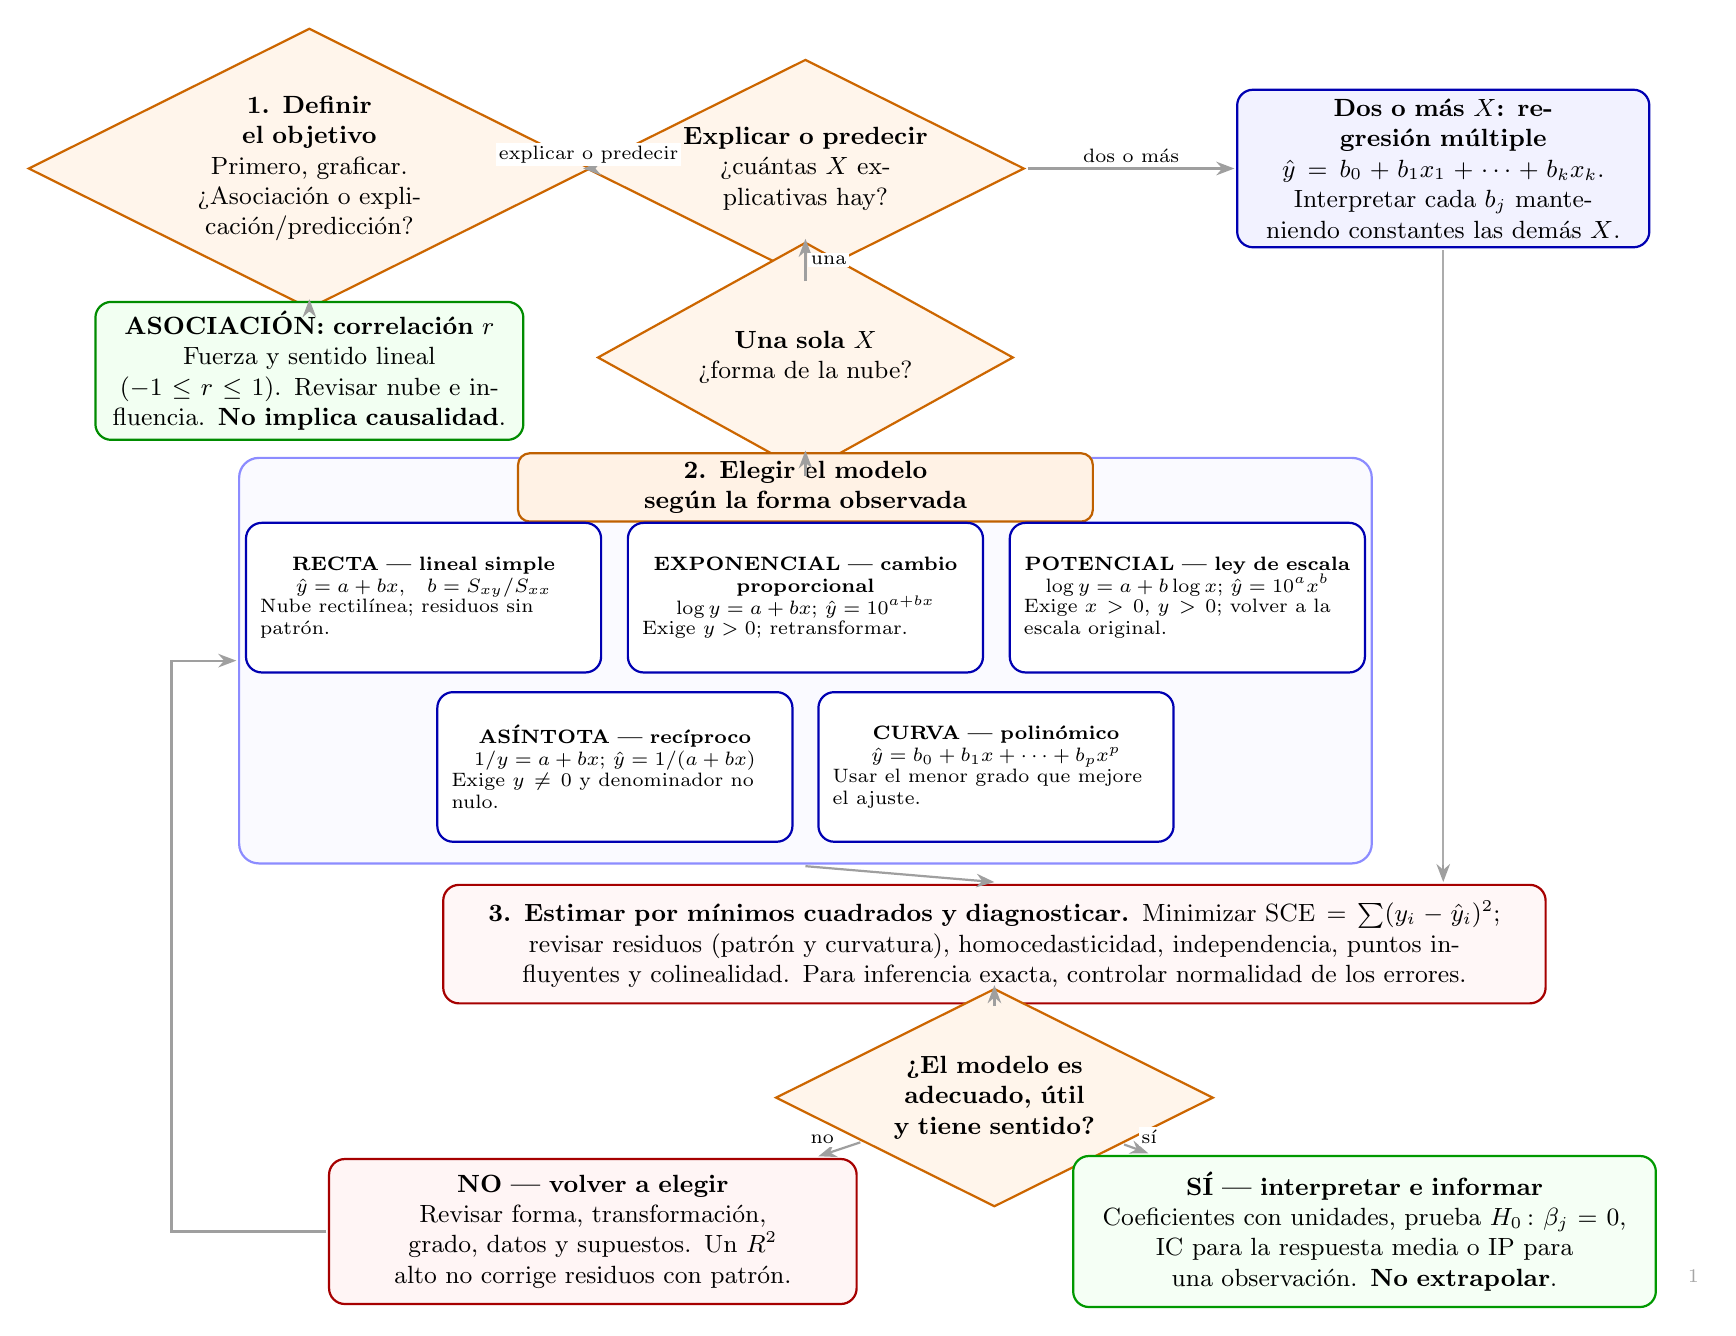
\begin{tikzpicture}[
  font=\small,
  decisionfinal/.style={diamond,aspect=2,draw=orange!80!black,fill=orange!8,
    thick,text width=3.15cm,align=center,inner sep=1.5pt},
  modelo/.style={rectangle,rounded corners=2mm,draw=blue!70!black,
    fill=white,thick,text width=4.15cm,minimum height=1.9cm,
    align=left,inner sep=1.8mm,font=\scriptsize},
  panel/.style={rectangle,rounded corners=2.5mm,draw=blue!45,
    fill=blue!2,thick,text width=14.15cm,minimum height=5.15cm},
  cabecera/.style={rectangle,rounded corners=1.5mm,draw=orange!75!black,
    fill=orange!10,thick,text width=7.1cm,minimum height=0.62cm,
    align=center,inner sep=1mm,font=\small},
  diagnostico/.style={rectangle,rounded corners=2mm,draw=red!65!black,
    fill=red!3,thick,text width=13.6cm,minimum height=1.45cm,
    align=center,inner sep=2mm,font=\small},
  salida/.style={rectangle,rounded corners=2mm,draw=green!60!black,
    fill=green!4,thick,text width=7.0cm,minimum height=1.55cm,
    align=center,inner sep=2mm,font=\small},
  retroceso/.style={rectangle,rounded corners=2mm,draw=red!65!black,
    fill=red!4,thick,text width=6.3cm,minimum height=1.55cm,
    align=center,inner sep=2mm,font=\small},
  bus/.style={thick,draw=gray!65},
  every node/.style={outer sep=1pt}
]

% 1. Objetivo y cantidad de variables
\node[decisionfinal] (objetivo) at (-8.7,0)
  {\textbf{1. Definir el objetivo}\\Primero, graficar.\\¿Asociación o explicación/predicción?};
\node[resultado,text width=5.2cm,minimum height=1.35cm,font=\small] (corr) at (-8.7,-2.57)
  {\textbf{ASOCIACIÓN: correlación $r$}\\Fuerza y sentido lineal ($-1\le r\le1$). Revisar nube e influencia. \textbf{No implica causalidad}.};
\node[decisionfinal] (nvar) at (-2.4,0)
  {\textbf{Explicar o predecir}\\¿cuántas $X$ explicativas hay?};
\node[proceso,text width=5.0cm,minimum height=1.6cm,font=\small] (multiple) at (5.7,0)
  {\textbf{Dos o más $X$: regresión múltiple}\\$\hat y=b_0+b_1x_1+\cdots+b_kx_k$. Interpretar cada $b_j$ manteniendo constantes las demás $X$.};
\node[decisionfinal,text width=3.8cm,aspect=1.8] (forma) at (-2.4,-2.40)
  {\textbf{Una sola $X$}\\¿forma de la nube?};

\draw[flujo] (objetivo)--(corr);
\draw[flujo] (objetivo)--node[etiqueta,above]{explicar o predecir}(nvar);
\draw[flujo] (nvar)--node[etiqueta,above]{dos o más}(multiple);
\draw[flujo] (nvar)--node[etiqueta,right]{una}(forma);

% 2. Selector compacto de modelos para una X
\node[panel] (modelpanel) at (-2.4,-6.25) {};
\node[cabecera] (modelhead) at (-2.4,-4.05)
  {\textbf{2. Elegir el modelo según la forma observada}};

\node[modelo] (lineal) at (-7.25,-5.45)
  {\centering\textbf{RECTA --- lineal simple}\\
   $\hat y=a+bx$,\quad $b=S_{xy}/S_{xx}$\\[-0.2mm]
   \raggedright Nube rectilínea; residuos sin patrón.};
\node[modelo] (exp) at (-2.4,-5.45)
  {\centering\textbf{EXPONENCIAL --- cambio proporcional}\\
   $\log y=a+bx$; $\hat y=10^{a+bx}$\\[-0.2mm]
   \raggedright Exige $y>0$; retransformar.};
\node[modelo] (pot) at (2.45,-5.45)
  {\centering\textbf{POTENCIAL --- ley de escala}\\
   $\log y=a+b\log x$; $\hat y=10^a x^b$\\[-0.2mm]
   \raggedright Exige $x>0$, $y>0$; volver a la escala original.};
\node[modelo] (rec) at (-4.82,-7.60)
  {\centering\textbf{ASÍNTOTA --- recíproco}\\
   $1/y=a+bx$; $\hat y=1/(a+bx)$\\[-0.2mm]
   \raggedright Exige $y\ne0$ y denominador no nulo.};
\node[modelo] (poli) at (0.02,-7.60)
  {\centering\textbf{CURVA --- polinómico}\\
   $\hat y=b_0+b_1x+\cdots+b_px^p$\\[-0.2mm]
   \raggedright Usar el menor grado que mejore el ajuste.};

\draw[flujo] (forma)--(modelhead);

% 3. Estimación y diagnóstico comunes
\node[diagnostico] (diagnostico) at (0,-9.85)
  {\textbf{3. Estimar por mínimos cuadrados y diagnosticar.}
   Minimizar $\mathrm{SCE}=\sum(y_i-\hat y_i)^2$; revisar residuos (patrón y curvatura),
   homocedasticidad, independencia, puntos influyentes y colinealidad.
   Para inferencia exacta, controlar normalidad de los errores.};

\draw[flujo] (modelpanel.south)--(diagnostico.north);
\coordinate (multjoin) at (5.7,-8.85);
\draw[bus] (multiple.south)--(multjoin);
\draw[flujo] (multjoin)--(multjoin |- diagnostico.north);

% 4. Decisión posterior al diagnóstico
\node[decisionfinal] (adecuado) at (0,-11.80)
  {\textbf{¿El modelo es adecuado, útil y tiene sentido?}};
\node[retroceso] (revisar) at (-5.1,-13.50)
  {\textbf{NO --- volver a elegir}\\Revisar forma, transformación, grado, datos y supuestos. Un $R^2$ alto no corrige residuos con patrón.};
\node[salida] (informar) at (4.7,-13.50)
  {\textbf{SÍ --- interpretar e informar}\\Coeficientes con unidades, prueba $H_0\!:\beta_j=0$, IC para la respuesta media o IP para una observación. \textbf{No extrapolar}.};

\draw[flujo] (diagnostico)--(adecuado);
\draw[flujo] (adecuado)--node[etiqueta,above left]{no}(revisar);
\draw[flujo] (adecuado)--node[etiqueta,above right]{sí}(informar);
\draw[flujo] (revisar.west) -| (-10.45,-6.25) -- (modelpanel.west);

\node[anchor=south east,font=\scriptsize,text=gray!70] at (9.1,-14.30) {\thepage};

\end{tikzpicture}
}
\end{center}
\end{paisaje}

\end{document}
